\chapter{Anharmonischer Oszillator\label{chapter:anharmonisch}}
\lhead{Anharmonischer Oszillator}
\begin{refsection}
\chapterauthor{Joel Brunner und Christian Cavegn}

In diesem Kapitel erweitern wir den harmonischen Oszillator aus
Kapitel~\ref{chapter:harmonischeroszillator} mit Hilfe der St"orungstheorie aus
Kapitel~\ref{chapter:stoerungstheorie}.
Der harmonische Oszillator ist eine gute Approximation f"ur viele
Quantenmechanische Systeme.
Will man die Approximation verbessern,
kann man die Kr"afte im Oszillator nicht mehr linear modellieren.
Das Potential ist also nicht mehr nur $Q^2$,
sondern es kommen noch Terme h"oherer Ordnung hinzu.
Beziehungsweise Konstanten wie in Kapitel~\ref{chapter:efeld} zu sehen ist.
Diese Terme k"onnen als St"orungen betrachtet werden.
Wir betrachten in diesem Kapitel nur Zeitunabh"angige und nicht entartete
St"orungen, da alles Andere den Rahmen sprengen w"urde.

\begin{figure}	%Bild Titelbild.png
\centering
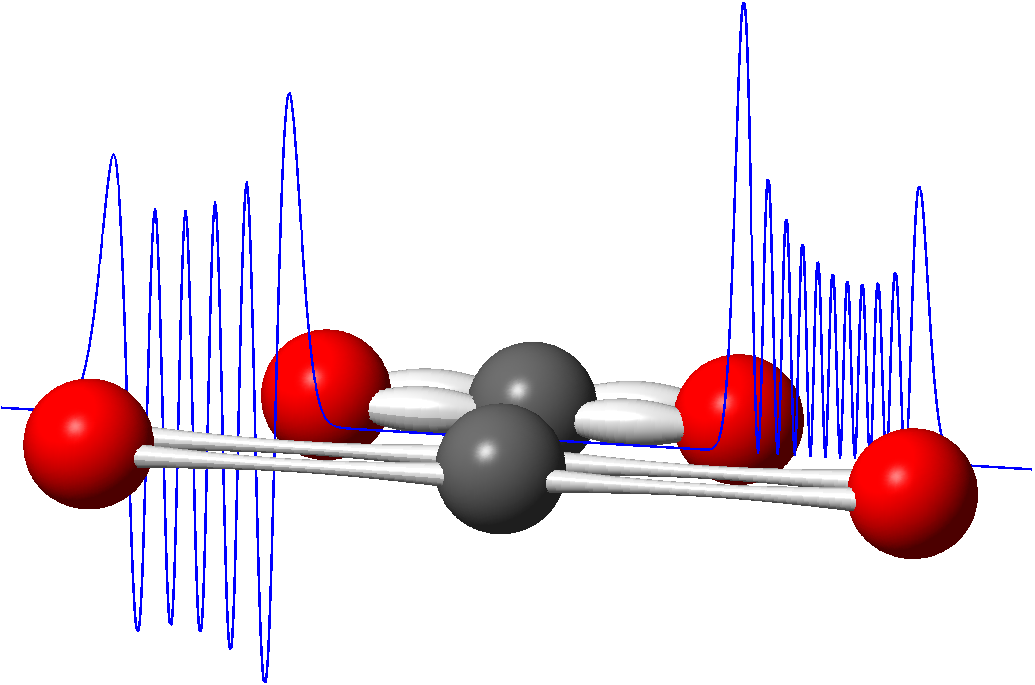
\includegraphics[width=0.7\textwidth]{anharmonisch/images/Titelbild.png}
\caption{Beispiel einer symmetrischen Valenzschwingung eines Kohlendioxid Molek"uls
\label{skript:Titelbild}}
\end{figure}

			%Anharmonizit"at
\section{Anharmonizit"at}
\rhead{Anharmonizit"at}

\begin{figure}	%Bild Potentiale
\centering
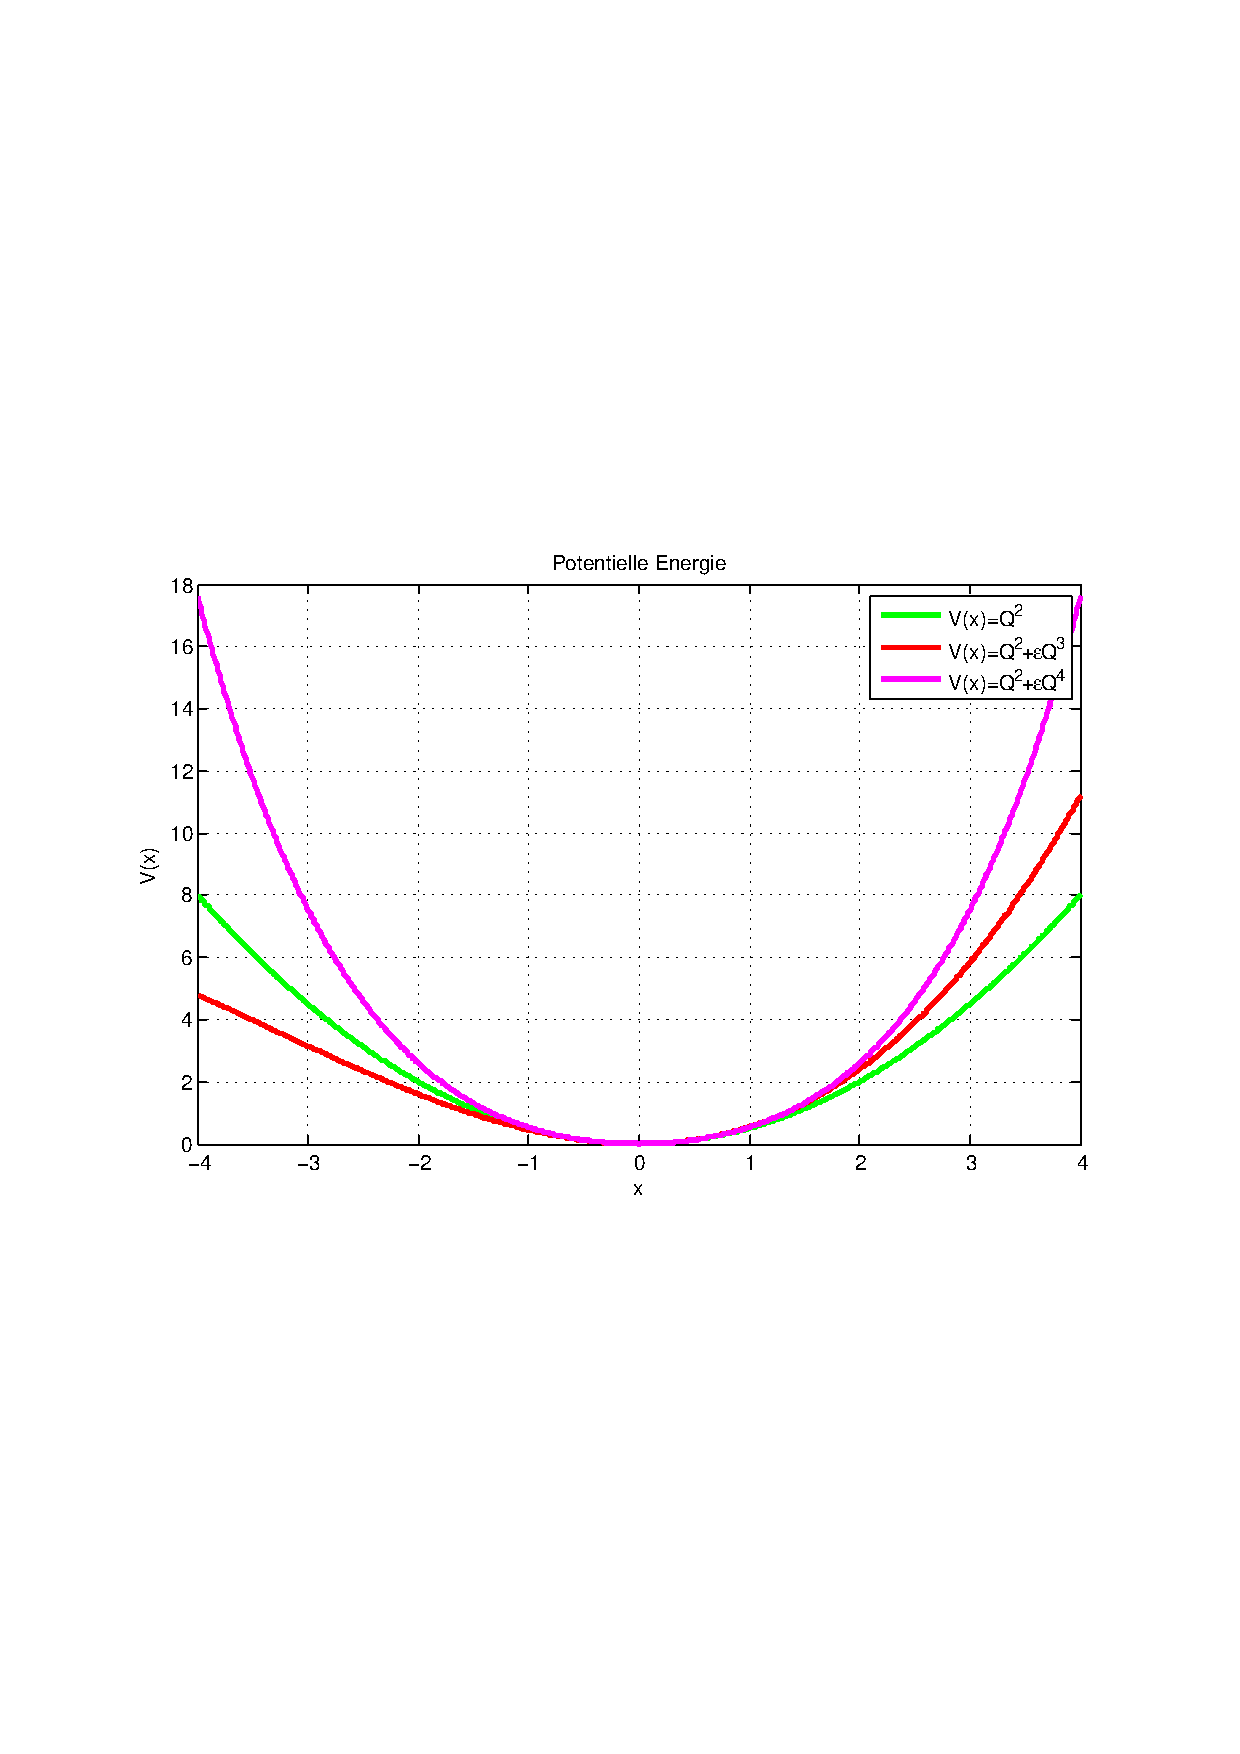
\includegraphics[width=0.7\textwidth]{anharmonisch/images/Potential.pdf}
\caption{Potentiale eines harmonischen und anharmonischen Oszillators
\label{skript:Potentiale}}
\end{figure}

\[
H(p,x)
=
\underbrace{\frac1{2m}p^2+\frac12 kx^2}_{H_0}
\underbrace{\vphantom{\frac1{2m}p^2+\frac12 kx^2}
+a_3 x^3+a_4 x^4+a_5 x^5+\dotsb}_{\varepsilon H_1}
\]

Auf der Abbildung~\ref{skript:Potentiale} sieht man das Potential der mit
$Q^3$ oder $Q^4$ gest"orten Oszillatoren im Vergleich zum harmonischen Oszillator.
Das System ist linear und wurde in
Kapitel~\ref{chapter:harmonischeroszillator} vollst"andig gel"ost.
Rechts sieht man das Potential des gest"orten Oszillators.
Es wird durch "aussere und innere Kraftfelder,
wie zum Beispiel der Coulombkraft oder dem Gravitationsfeld gest"ort.
In diesem Fall sind zus"atzlich noch Terme wie $Q^3$ oder $Q^4$ im Potential enhalten.

			%St"orungstheorie
\section{St"orungstheorie}
\rhead{St"orungstheorie}
F"ur unsere Berechnungen gehen wir von dieser Schr"odingergleichung aus.
\begin{equation}
(H_0+\varepsilon H_1)|\Psi_k(\varepsilon)\rangle
=
E_k(\varepsilon)|\Psi_k(\varepsilon)\rangle
\end{equation}
Mit den Koeffizienten
\begin{align*}
E_k(\varepsilon)
&=
E_k^{(0)}+\varepsilon E_k^{(1)}+\varepsilon^2 E_k^{(2)}+\dotsb
\\
|\Psi_k(\varepsilon)\rangle
&=
|\Psi_k^{(0)}\rangle+\varepsilon|\Psi_k^{(1)}\rangle+
\varepsilon^2|\Psi_k^{(2)}\rangle+\dotsb
\end{align*}
Durch Ausmultiplizieren,
wie in Abschnitt~\ref{section:nichtentartetezustaende} beschrieben,
kommt man auf folgende generische Gleichungen, mit
\[
C_{lk}^{(p)}
=
\displaystyle\sum_{j=2}^{p} E_k^{(p-j-1)}
\langle\Psi_l^{(0)}|\Psi_k^{(j-1)}\rangle
\]
\begin{equation}
\begin{aligned}
\langle\Psi_l^{(0)}|\Psi_k^{(p)}\rangle
&=
\frac{C_{lk}^{(p)}-\langle\Psi_l^{(0)}|H_1|\Psi_k^{(p-1)}\rangle}
{E_k^{(0)}-E_l^{(0)}}
\text{mit}
l&\ne k
\\
E_k^{(p)}
&=
\langle\Psi_l^{(0)}|H_1|\Psi_l^{(k)}\rangle-C_{lk}^{(p)}
\end{aligned}
\end{equation}
Das ist eine rekursive Formel.
Das bedeutet, dass aus den vorherigen St"orkoeffizienten,
die nachfolgenden berechnet werden k"onnen.
F"ur die noch fehlenden Skalarprodukte $\langle\Psi_k^{(0)}|\Psi_l^{(0)}\rangle$
mit $k=l$ sehen wir und die Normierung nochmals genauer an.
\[
\langle\Psi_k|\Psi_k\rangle=1
\]
Mit Hilfe der Bedingung
\[
\langle\Psi_a|\Psi_b\rangle
=
\langle\Psi_b|\Psi_a\rangle^*,
\]
erhalten wir die Werte f"ur die gesuchten Skalare.
Denn die Koeffizienten der Epsilons m"ussen Null ergeben, damit die Normierung gilt.
\begin{align*}
1
=
&\underbrace{\langle\Psi_k^{(0)}|\Psi_k^{(0)}\rangle}_{=1}
\\
&+\varepsilon\bigl(\langle\Psi_k^{(0)}|\Psi_k^{(1)}\rangle
+\langle\Psi_k^{(1)}|\Psi_k^{(0)}\rangle\bigr)
\\
&+\varepsilon^2\bigl(\langle\Psi_k^{(0)}|\Psi_k^{(2)}\rangle
+\langle\Psi_k^{(1)}|\Psi_k^{(1)}\rangle
+\langle\Psi_k^{(2)}|\Psi_k^{(0)}\rangle\bigr)
\\
&+\varepsilon^3\bigl(\langle\Psi_k^{(0)}|\Psi_k^{(3)}\rangle
+\langle\Psi_k^{(1)}|\Psi_k^{(2)}\rangle
+\langle\Psi_k^{(2)}|\Psi_k^{(1)}\rangle
+\langle\Psi_k^{(3)}|\Psi_k^{(0)}\rangle\bigr)
\\
&+\varepsilon^4\bigl(\langle\Psi_k^{(0)}|\Psi_k^{(4)}\rangle
+\langle\Psi_k^{(1)}|\Psi_k^{(3)}\rangle
+\langle\Psi_k^{(2)}|\Psi_k^{(2)}\rangle
+\langle\Psi_k^{(3)}|\Psi_k^{(1)}\rangle
+\langle\Psi_k^{(4)}|\Psi_k^{(0)}\rangle\bigr)
\end{align*}
Dadurch erhalten wir
\begin{equation}
l=k
\Rightarrow
\langle\Psi_l^{(0)}|\Psi_k^{(p)}\rangle
=
i\gamma_p+
\frac12 \displaystyle\sum_{j=2}^{p} 
\langle\Psi_k^{(p-j+1)}|\Psi_k^{(j-1)}\rangle
\end{equation}
$\gamma_p$ muss so gew"ahlt werden, dass die Wellenfunktion in p-ter N"aherung stimmt.
%\[
%\langle\Psi_k^{(p)}|\Psi_k^{(p)}\rangle=1
%\]
Das Skalarprodukt beschreibt die Abh"angigkeit zweier Vektoren.
Um sich eine bessere Vorstellung zu verschaffen, dient die Gleichung
\[
|\langle\Psi_l^{(0)}|\Psi_k^{(p)}\rangle|^2
=
P(\Psi_l^{(0)}|\Psi_k^{(p)}),
\]
welche aussagt, wie wahrscheinlich es ist,
dass die ungest"orte Wellenfunktion $|\Psi_l^{(0)}\rangle$
in der Zustandskorrektur $|\Psi_k^{(p)}\rangle$ vorkommt.
\begin{equation}
|\Psi_k^{(p)}\rangle
=
\displaystyle\sum_{l=0}^{\infty}
\underbrace{\langle\Psi_l^{(0)}|\Psi_k^{(p)}\rangle}_{\text{Koeffizienten}}
|\Psi_l^{(0)}\rangle
\end{equation}

			%Implemeintation
\section{Implementation}
\rhead{Implementation}

\begin{figure}	%Bild Harmonisch.pdf
\centering
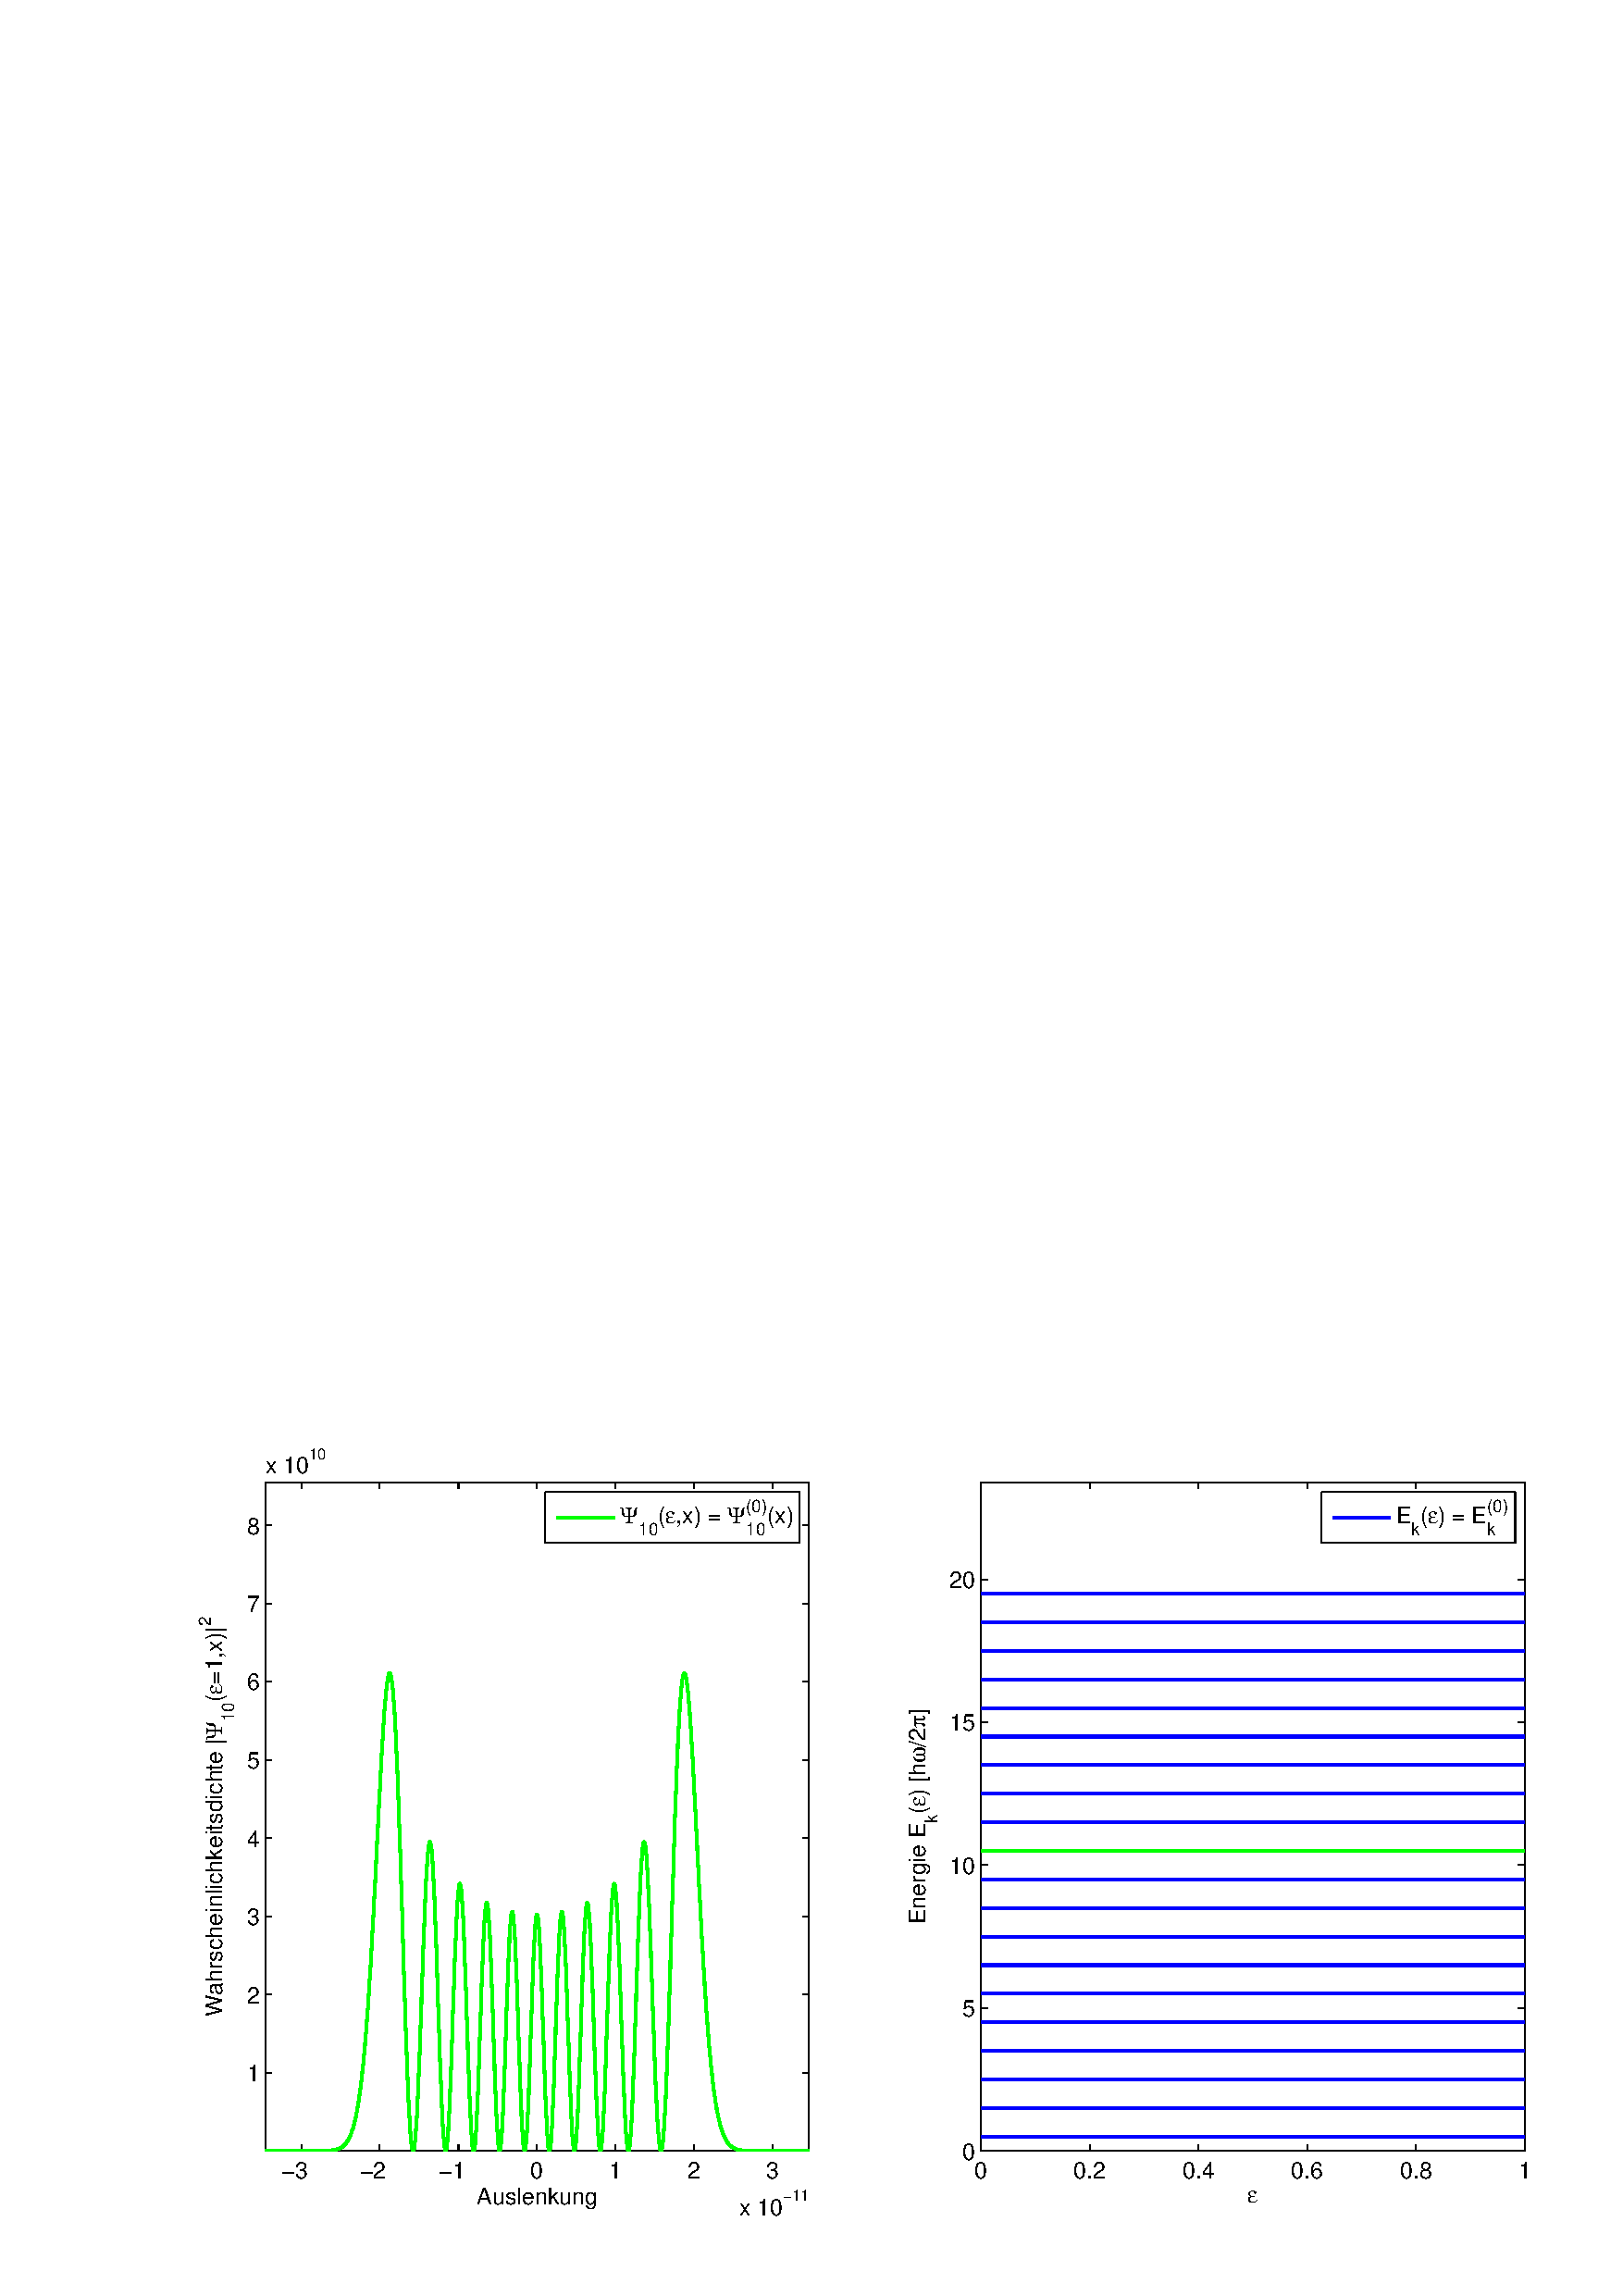
\includegraphics[width=0.7\textwidth]{anharmonisch/images/Harmonisch.pdf}
\caption{10. Wellenfunktion und Energieniveaus des harmonischen Oszillators
\label{skript:Harmonisch}}
\end{figure}

Der Grundzustand (\ref{skript:grundzustandwellenfunktion})
hat die Form einer Gausskurve.
F"ur die Implementierung und Optimierung leiten wir eine Form der Wellenfunktion her,
bei welcher wir die $e$-Funktion nur einmal ausrechnen m"ussen.
Das erm"oglicht eine deutlich k"urzere Berechnungszeit.
Mit der geeigneten Normierung bekommen wir den Grundzustand
\[
\Psi_0(x)
=
\biggl(\frac{m\omega}{\pi\hbar}\biggr)^\frac14
e^{-\frac12\frac{m\omega}{\hbar}x^2}.
\]
Aus der Gleichung
\[
|n\rangle
=
\frac{1}{\sqrt{N_n}}(a^+)^n\,|0\rangle
\]
wird die Iterationsformel
\begin{equation}
\Psi_k(x)
=
\frac1{\sqrt{k!}}\biggl(\frac1{\sqrt{2}}
\biggl(\sqrt{\frac{m\omega}{\hbar}x}-
\sqrt{\frac{\hbar}{m\omega}}\frac{\partial}{\partial x}\biggr)\biggr)^k
\biggl(\frac{m\omega}{\pi\hbar}\biggr)^\frac14
e^{-\frac12\frac{m\omega}{\hbar}x^2}
\label{skript:iterationsformel}
\end{equation}
abgeleitet.
In die Gleichung substituiert man
\[
\alpha=\sqrt{\frac{m\omega}\hbar}
\]
und formt sie ein wenig um.
\[
\Psi_k(x)
=
\frac1{\sqrt{k!}}\frac1{\sqrt{2^k}}
\biggl(\frac{m\omega}{\pi\hbar}\biggr)^\frac14
\biggl(\alpha x-\frac1{\alpha}\frac{\partial}{\partial x}\biggr)^k
e^{-\frac12\alpha^2x^2}
\]
Durch Ausmultiplizieren der Differentialgleichung erhalten wir ein Polynom,
welches f"ur die numerische Berechnung sehr hilfreich sein wird.
\begin{align*}
\biggl(\alpha x-\frac1{\alpha}\frac{\partial}{\partial x}\biggr)
e^{-\frac12\alpha^2x^2}
&=
(2\alpha x)e^{-\frac12\alpha^2x^2}
\\
&=
H_1(x)e^{-\frac12\alpha^2x^2}
\Rightarrow
H_1(x)
=
2ax
\\
\biggl(\alpha x-\frac1{\alpha}\frac{\partial}{\partial x}\biggr)^2
e^{-\frac12\alpha^2x^2}
&=
\biggl(\alpha x-\frac1{\alpha}\frac{\partial}{\partial x}\biggr)
(2\alpha x)e^{-\frac12\alpha^2x^2}
\\
&=
\biggl(2\alpha^2 x^2-2\frac{\partial}{\partial x}x\biggr)
e^{-\frac12\alpha^2x^2}
\\
&=
(2\alpha^2x^2-(2-2\alpha^2x^2))e^{-\frac12\alpha^2x^2}
\\
&=
(4\alpha^2x^2-2)e^{-\frac12\alpha^2x^2}
\\
&=
H_2(x)e^{-\frac12\alpha^2x^2}
\Rightarrow
H_2(x)
=
4a^2x^2-2
\end{align*}
Man erh"alt die Hermitpolynome $H_k$,
welche sich mit der Substitution
\[
z
=
ax.
\]
noch weiter vereinfachen lassen.
\[
H_k(z)
=
e^{\frac{z^2}2}\biggl(z-\frac{\partial}{\partial z}\biggr)^k
e^{-\frac{z^2}2}.
\]
Dadurch wird die Gleichung~\ref{skript:iterationsformel} gek"urzt zu
\begin{equation}
\Psi_k(z)
=
\biggl(\frac{m\omega}{\pi\hbar}\biggr)^\frac14
\frac1{\sqrt{2^k k!}}H_k(z)
e^{-\frac12 z^2}
\end{equation}
Der Vorteil dieser Notation ist die sehr einfache Implementierung
in den g"angigsten Berechnungtools.
Da die $e$-Funktion bereits ausgeklammert wurde, verk"urzt sich die Rechenzeit
signifikant.
%\begin{table}
%\centering
%\begin{tabular}{|l|l|}
%\hline
%$H_0 (z)$ & $1$				\\ \hline
%$H_1 (z)$ & $2z$				\\ \hline
%$H_2 (z)$ & $4z^2-2$				\\ \hline
%$H_3 (z)$ & $8z^3-12z$				\\ \hline
%$H_4 (z)$ & $16z^4-48z^2+12$			\\ \hline
%\end{tabular}
%\caption{Liste mit den ersten f"unf Hermitpolynomen\label{skript:Hermitpolynom}}
%\end{table}

\subsection{Tipps zur numerischen Berechnung}
F"ur die Interessierten unter den Lesern,
welche diese St"orungstheorie anwenden wollen,
m"ochten wir noch einige Tipps auf den Weg geben.
Wie ihr bereits erkennen konntet,
ist die Berechnung der  Ungest"orten Funktionen oft bereits sehr Rechenintensiv.
Aus diesem Grund,
empfiehlt es hier einer numerischen Auswertung der St"orungstheorie zu machen.
Dadurch verlagert sich die Berechnungsschwerpunkt
haupts"achlich auf die $\Psi^{((0))}$ Funktionen.
Wir schlagen aus diesem Grund,
im Falle des Harmonischen Oszillators, die folgender Matrixform vor.
\[
\Psi^{(0)}
=
\begin{pmatrix}
\Psi_0^{(0)}(x_0) & \cdots & \Psi_0^{(0)}(x_m)	\\
\Psi_1^{(0)}(x_0) & \cdots & \Psi_1^{(0)}(x_m)	\\
\vdots & \ddots & \vdots			\\
\Psi_n^{(0)}(x_0) & \cdots & \Psi_n^{(0)}(x_m)	\\
\end{pmatrix}
\]
Da die  Aufenthaltswahrscheinlichkeit eines Teilchens,
ausserhalb der Energiebarriere aus Abbildung~\ref{skript:Potentiale},
exponentiell abnimmt,
k"onnen wir die Wellenfunktionen mit einem endlichen Bereich beschreiben.
Zu beachten ist,
dass man immer mit dem gr"osstm"oglichen Bereich arbeiten sollte.
Im Falle des harmonischen Oszillators ist es der Bereich jenes Teilchens,
welches sich im h"ochstm"oglichen Energieniveau befindet.
Durch seine Energie oszilliert es weiter vom Arbeitspunkt weg
als ein Teilchen geringerer Energie.
Daraus l"asst sich aus
\begin{align*} 
E_{\text{pot}}
&=
\frac12 kx^2
\\
E_k
&=
E_{\text{pot}}
\\
E_k
&=
\hbar\omega\biggl(k+\frac12\biggr)
\\
\hbar\omega(\frac12+n)
&=
\frac12 kx^2
\end{align*}
folgender Arbeitsbereich ermitteln.
\[
x
=
\pm\sqrt{\frac{2\hbar\omega(\frac12+k_{max})}k}
\]
Dieser Bereich ist jedoch noch zu klein gew"ahlt.
Denn die Wahrscheinlichkeit dass sich ein Teilchen
(speziell der h"oheren Energieniveaus) ausserhalb dieses Bereichs vorfinden ist,
ist immer noch gross.
Aus dieser Feststellung muss man den Bereich noch weiter vergr"ossern.
In unseren Berechnungen haben wir den Bereich um 25\% weiter vergr"ossert.
\[
x
=
\pm\sqrt{\frac{2\hbar\omega(\frac12+k_{max})}k}*1.25
\]
Die Wahrscheinlichkeit,
dass sich nun das Teilchen im n-ten Energieniveau in diesem Bereich aufh"alt,
ist ausreichend gross.


			%Auswertung
\section{Auswertung}
\rhead{Auswertung}

Wir haben den Fall $Q^3$ und $Q^4$ mit Matlab durchgerechnet und sind auf
ein paar interessante Erkenntnisse gestossen.
Auf den folgenden Abbildungen ist die stellen die Farbe gr"un
immer den ungest"orten Fall dar und rot den gest"orten.
Die Regenbogenfarben dienen in erster Linie dazu, den Verlauf von
tiefen Wellenfunktionen (blau) zu hohen Wellenfunktionen (rot) besser darzustellen.
Bei den Berechnungen haben wir die ersten 50 Wellenfunktionen und Energieniveaus
betrachtet.

			%Erstes Beispiel
\subsection{Erstes Beispiel $Q^4$}

\begin{figure}	%Bild Stoerung1Skalare.pdf
\centering
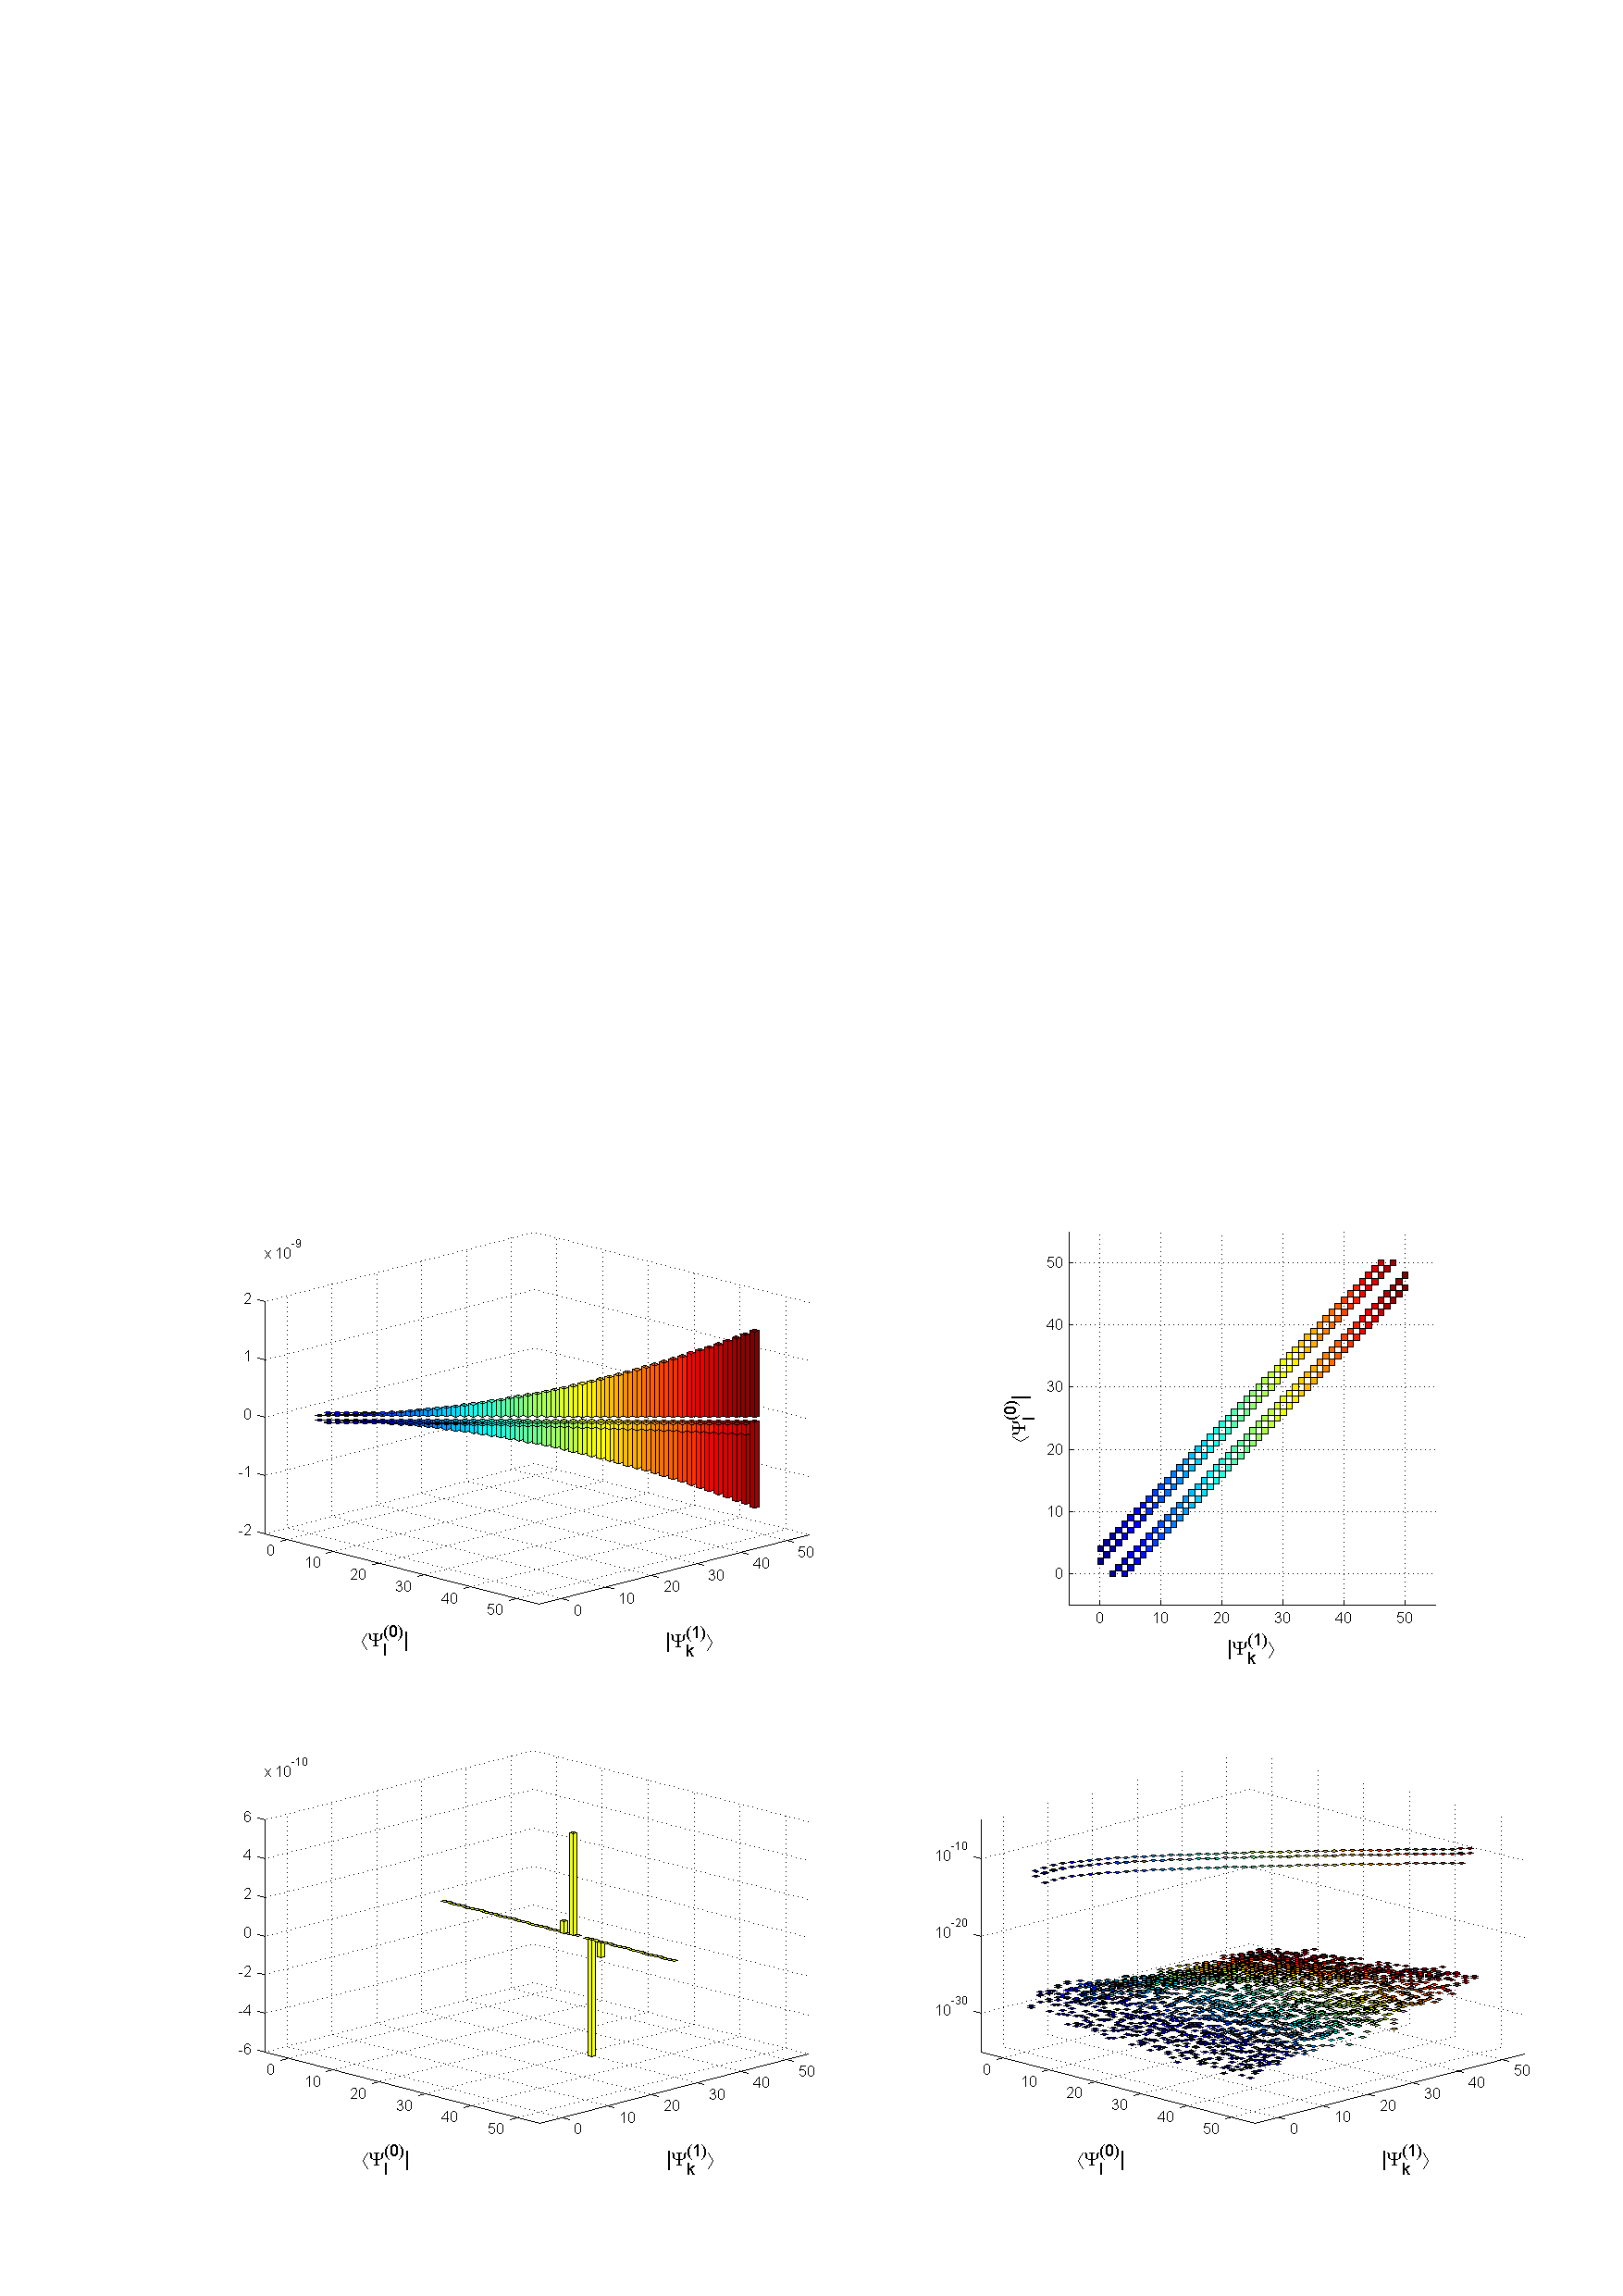
\includegraphics[width=1.0\textwidth]{anharmonisch/images/x4/Stoerung1Skalare.pdf}
\caption{$Q^4$ erster N"aherung: Skalarprodukte $\langle\Psi_l^{(0)}|\Psi_k^{(1)}\rangle$
\label{skript:x4_Stoerung1Skalare}}
\end{figure}

Die Abbildung~\ref{skript:x4_Stoerung1Skalare} besteht aus vier Ansichten,
welche alle mit den Skalarprodukten der Wellenfunktionen zu tun haben.
Auf der Grafik oben rechts sieht man welche ungest"orten
Wellenfunktionen $\Psi_l^{(0)}$ den gr"ossten Anteil am
St"orterm $\Psi_k^{(1)}$ haben.
Das heisst, aus welchen bekannten Wellenfunktionen sich die neue Wellenfunktion
zusammensetzt.
Oben links sieht man die wie gross das Skalarprodukt ist, das heisst wie gross der
Anteil an der gest"orten Wellenfunktion ist.
Auf der Grafik unten links ist die 30. Wellenfunkion $\Psi_{30}^{(1)}$ separat,
mit allen Anteilen von ungest"orten Wellenfunktionen.
Das heisst auch den unbedeutenden Anteile.
Unten rechts ist eine logarithmische Darstellung, welche ebenfalls die unbedeutenden
Anteile zeigt. Diese Anteile wurden durch die numerische Berechnung erzeugt.
Nun zu den Besonderheiten von bei $Q^4$ in erster N"aherung.
Die Wellenfunktionen $\Psi_l^{(0)}$ welchen nahe bei der gest"orten Wellenfunktion
$\Psi_k^{(1)}$ sind haben den gr"ossten Anteil.
Dies war zu erwarten, da der Nenner der
Gleichung~\ref{skript:stoerungsloesung1ordnung} bei diesen am kleinsten ist.
Die Wellenfunktionen, bei welchen $l=k\pm 1,k\pm 3,\dots$ ist,
geben keinen Anteil an die gest"orte Wellenfunktion, da sie orthogonal dazu stehen.
Die Skalarprodukte sind bei $l<k$ positiv und bei $l>k$ negativ.
Das ist ebenfalls auf den Nenner der Gleichung~\ref{skript:stoerungsloesung1ordnung}
zur"uckzuf"uhren.
In der logarithmischen Darstellung sieht man, dass die Wellenfuntionen,
welche weiter weg sind nur noch einen vernachl"assigbar kleinen Beitrag liefern.
Grunds"atzlich ist aber auch dort eine Zunahme bei den h"oheren Wellenfunktionen
zu erkennen.

\begin{figure}	%Bild EK1.pdf
\centering
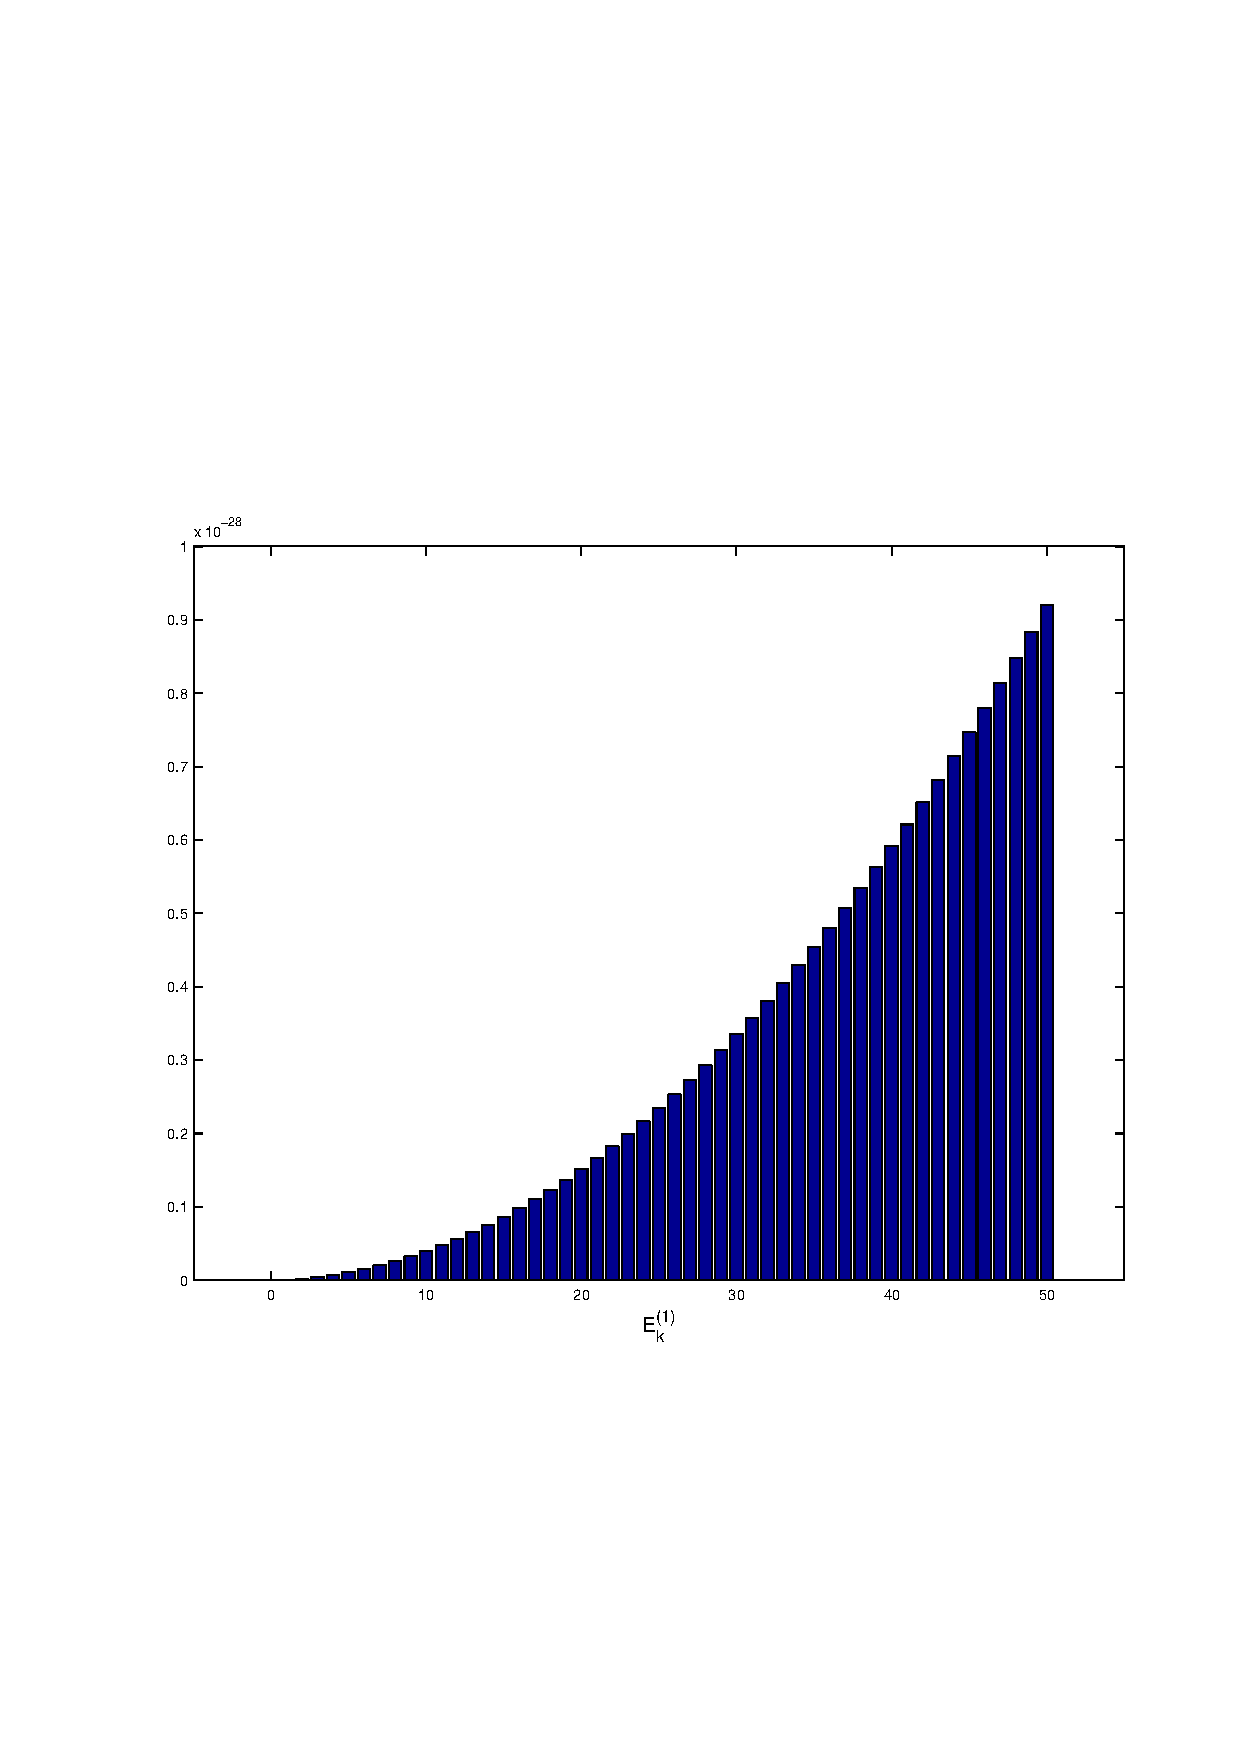
\includegraphics[width=0.7\textwidth]{anharmonisch/images/x4/EK1.pdf}
\caption{$Q^4$ erste N"aherung: St"orung der Energieniveaus
\label{skript:x4_EK1}}
\end{figure}

Die Abbildung~\ref{skript:x4_EK1} zeigt wie stark sich die Energieniveaus "andern,
im Vergleich zu den ungest"orten Energieniveaus.
In erster N"aherung sieht man sch"on, dass die tiefen Energieniveaus fast unver"andert
bleiben. Bei h"oheren Energieniveaus wird die Abweichung immer gr"osser.  

\begin{figure}	%Bild Stoerung1Wellenfunktion.pdf
\centering
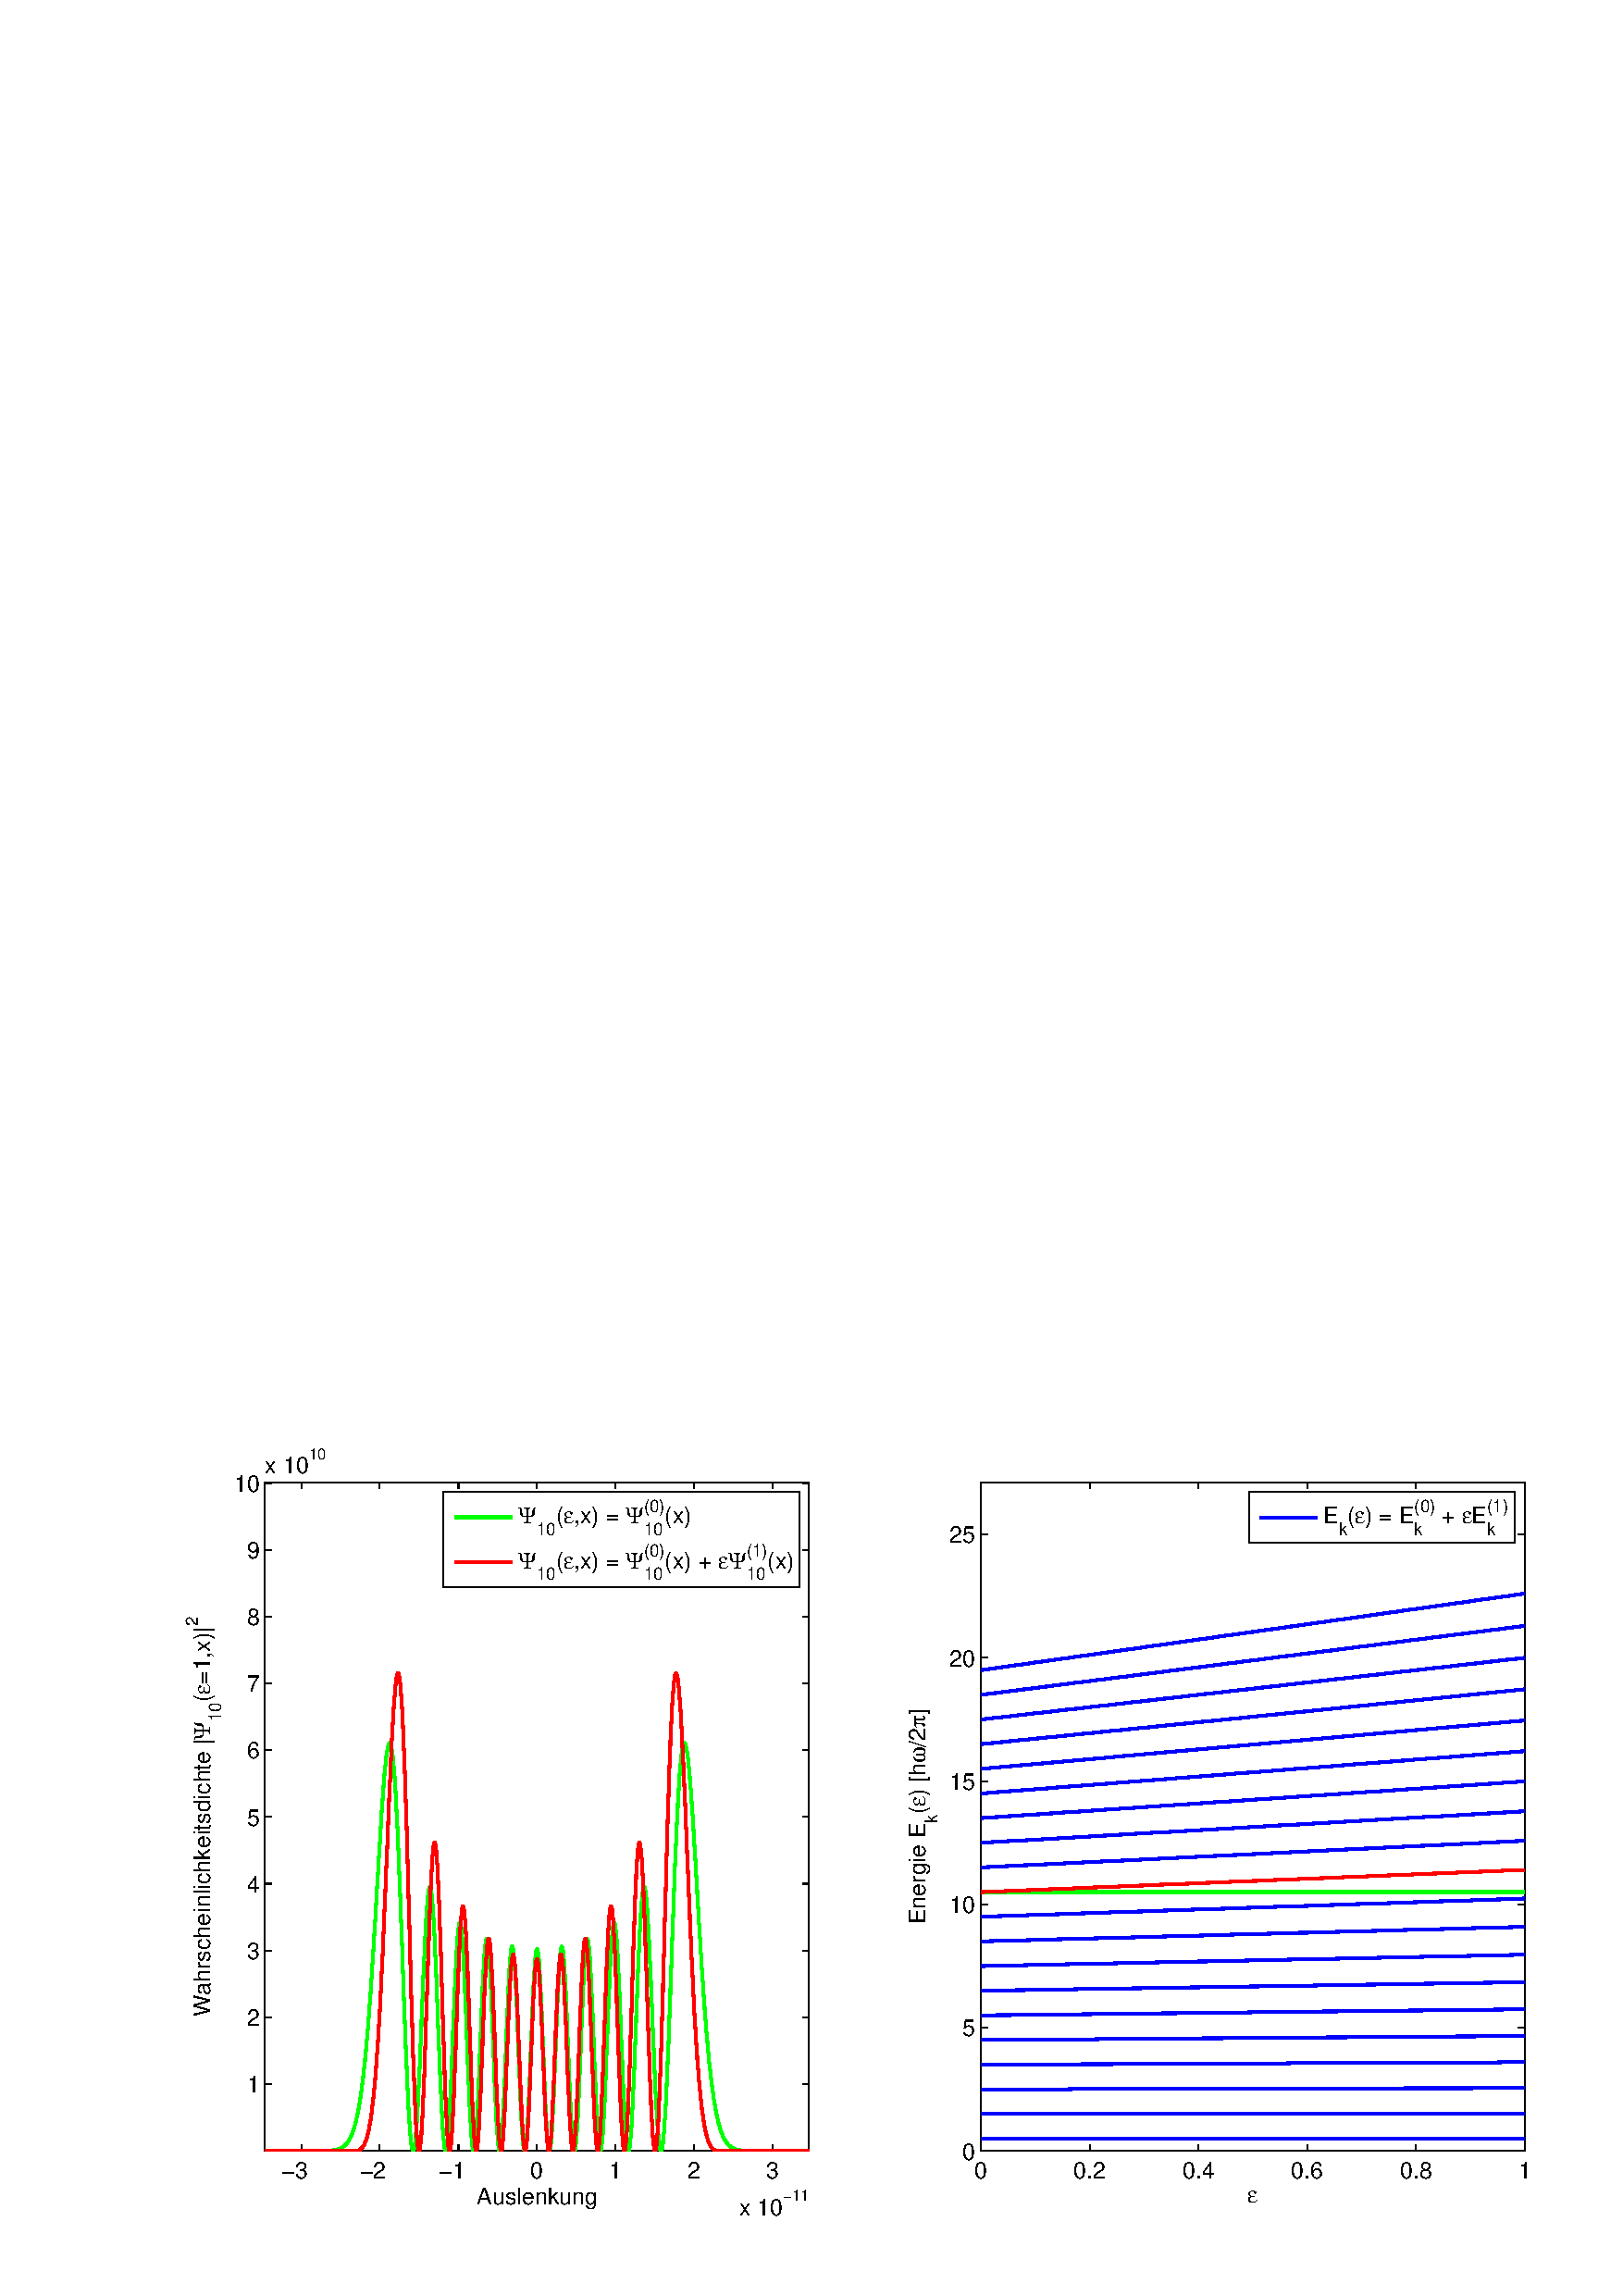
\includegraphics[width=0.8\textwidth]{anharmonisch/images/x4/Stoerung1Wellenfunktion.pdf}
\caption{$Q^4$ erster N"aherung: 10. Wellenfunktion und Energieniveaus
\label{skript:x4_Stoerung1Wellenfunktion}}
\end{figure}

Die Abbildung~\ref{skript:x4_Stoerung1Wellenfunktion} zeigt,
wie sich die St"orungen welche in Abbildung~\ref{skript:x4_Stoerung1Skalare} und
Abbildung~\ref{skript:x4_EK1} beschrieben wurden, auf die Wellenfunktionen und
Energieniveaus auswirken.
Auf der linken Grafik sieht man die 10. Wellenfunktion $\Psi_{10}$ in gest"orter und
und ungest"orter Form.
Auf der rechten Grafik sind die Energieniveaus in Abh"angigkeit von $\varepsilon$
zu sehen.
Das 10. Energieniveau ist ebenfalls farblich hervorgehoben.
In der ersten N"aherung wird die Wellenfunktion ein wenig zusammengedr"uckt.
Die Aufenthaltswahrscheinlichkeit ist bei gr"osseren Auslenkungen noch gr"osser
geworden als sie schon beim ungest"orten System ist.
Das kann bei Systemen beobachtet werden, bei welchen die Auslenkung in beiden
Richtungen begrenzt ist.
Zum Beispiel eine Feder welche sich bei zu grosser Auslenkung mechanisch verformt.
Bei tiefen Energieniveaus ist die Verschiebung noch sehr gering.
Bei h"oheren Energieniveau verschieben sie sich nach oben.
Die gest"orten Energieniveaus sind linear von $\varepsilon$ abh"angig.
Wird $\varepsilon$ gr"osser gemacht wird auch die St"orung gr"osser.


\begin{figure}	%Bild Stoerung2Skalare.pdf
\centering
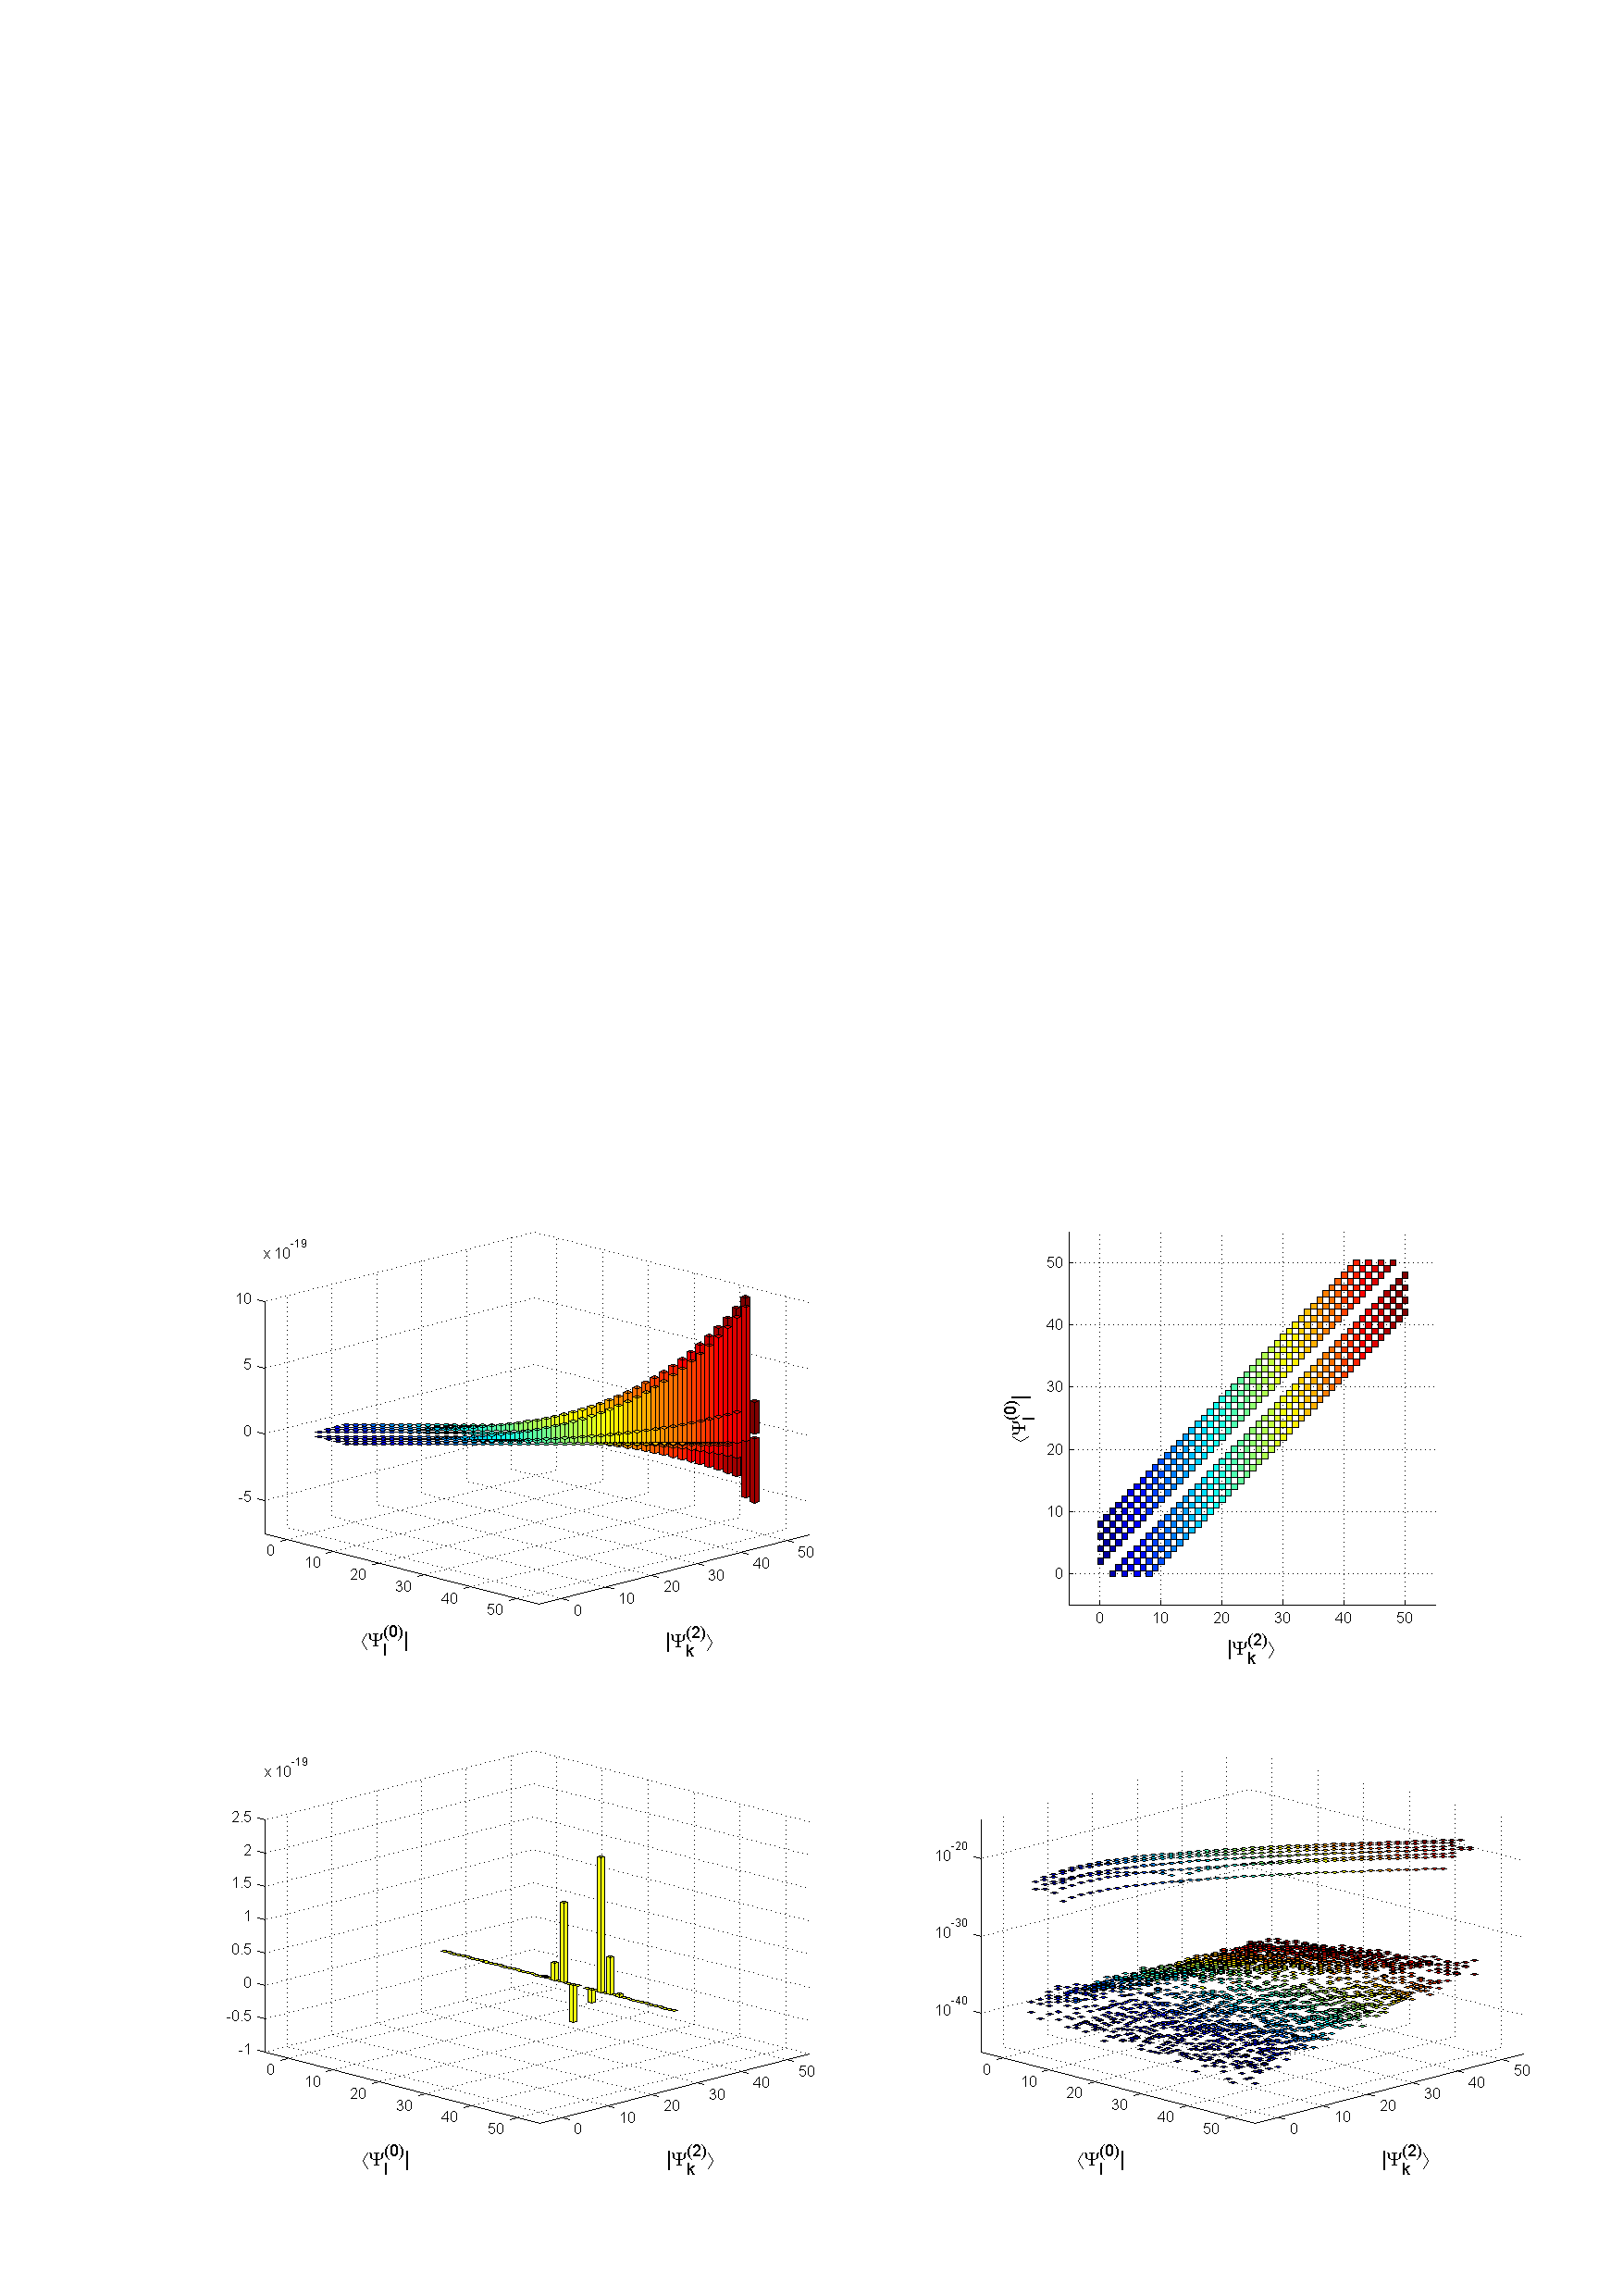
\includegraphics[width=1.0\textwidth]{anharmonisch/images/x4/Stoerung2Skalare.pdf}
\caption{$Q^4$ zweite N"aherung: Skalarprodukte $\langle\Psi_l^{(0)}|\Psi_k^{(2)}\rangle$
\label{skript:x4_Stoerung2Skalare}}
\end{figure}

Die Abbildung~\ref{skript:x4_Stoerung2Skalare} zeigt die zweite N"ahrung.
Wellenfunktionen, bei welchen $l=k\pm 1,k\pm 3,\dots$ ist,
geben keinen Anteil an die gest"orte Wellenfunktion.
Bei der zweiten N"aherung ist sind die Skalarprodukte zum gr"ossten Teil positiv,
da der Nenner der Gleichung immer positiv ist.
Wichtig ist auch zu beachten, dass f"ur die Berechnung dieser Werte die Werte von
der ersten N"aherung gebraucht werden.
Bei der Grafik oben rechts sieht man, dass Werte $>50$, welche von Wellenfunktionen
aus erster N"aherung stammen, f"ur die letzten acht Wellenfunktionen fehlen.
Dies "Aussert sich in Randeffekten. 


\begin{figure}	%Bild EK2.pdf
\centering
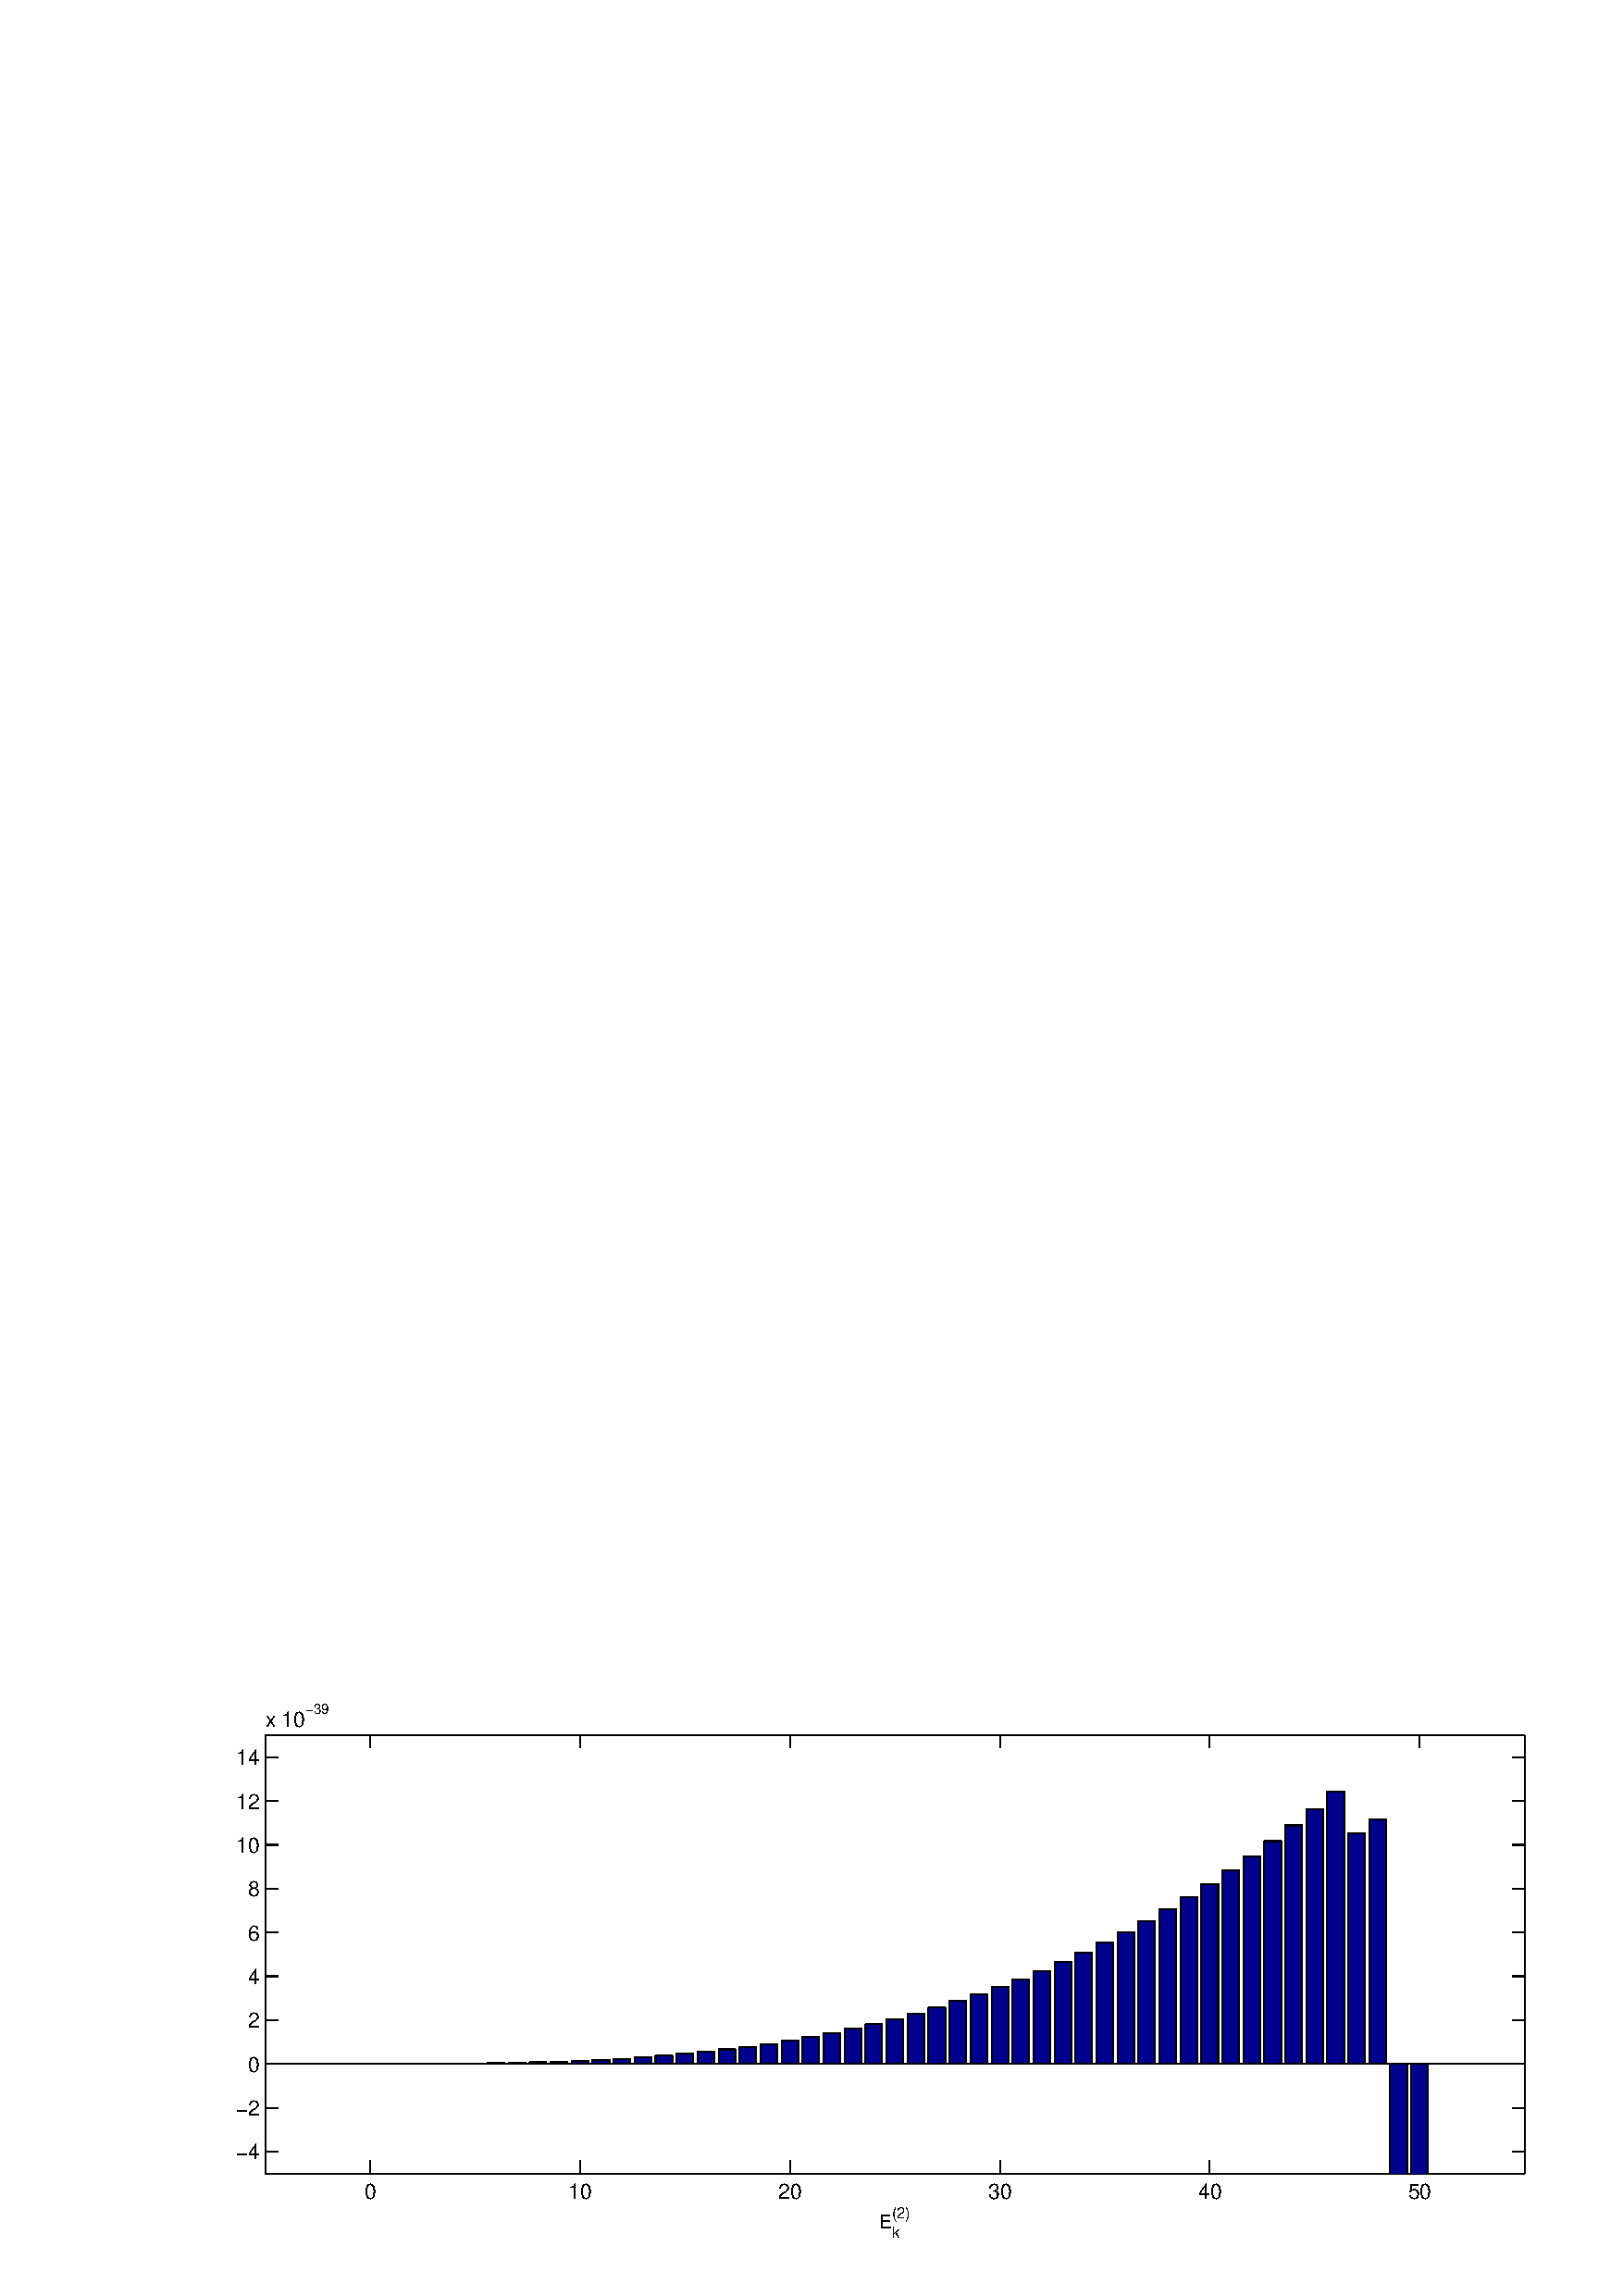
\includegraphics[width=0.7\textwidth]{anharmonisch/images/x4/EK2.pdf}
\caption{$Q^4$ zweite N"aherung: St"orung der Energieniveaus  
\label{skript:x4_EK2}}
\end{figure}

Auf der Abbildung~\ref{skript:x4_EK2} kann man die Randeffekte sehen.
Die letzten vier Energieniveaus m"ussen deshalb nicht beachtet werden.

\begin{figure}	%Bild Stoerung2Wellenfunktion.pdf
\centering
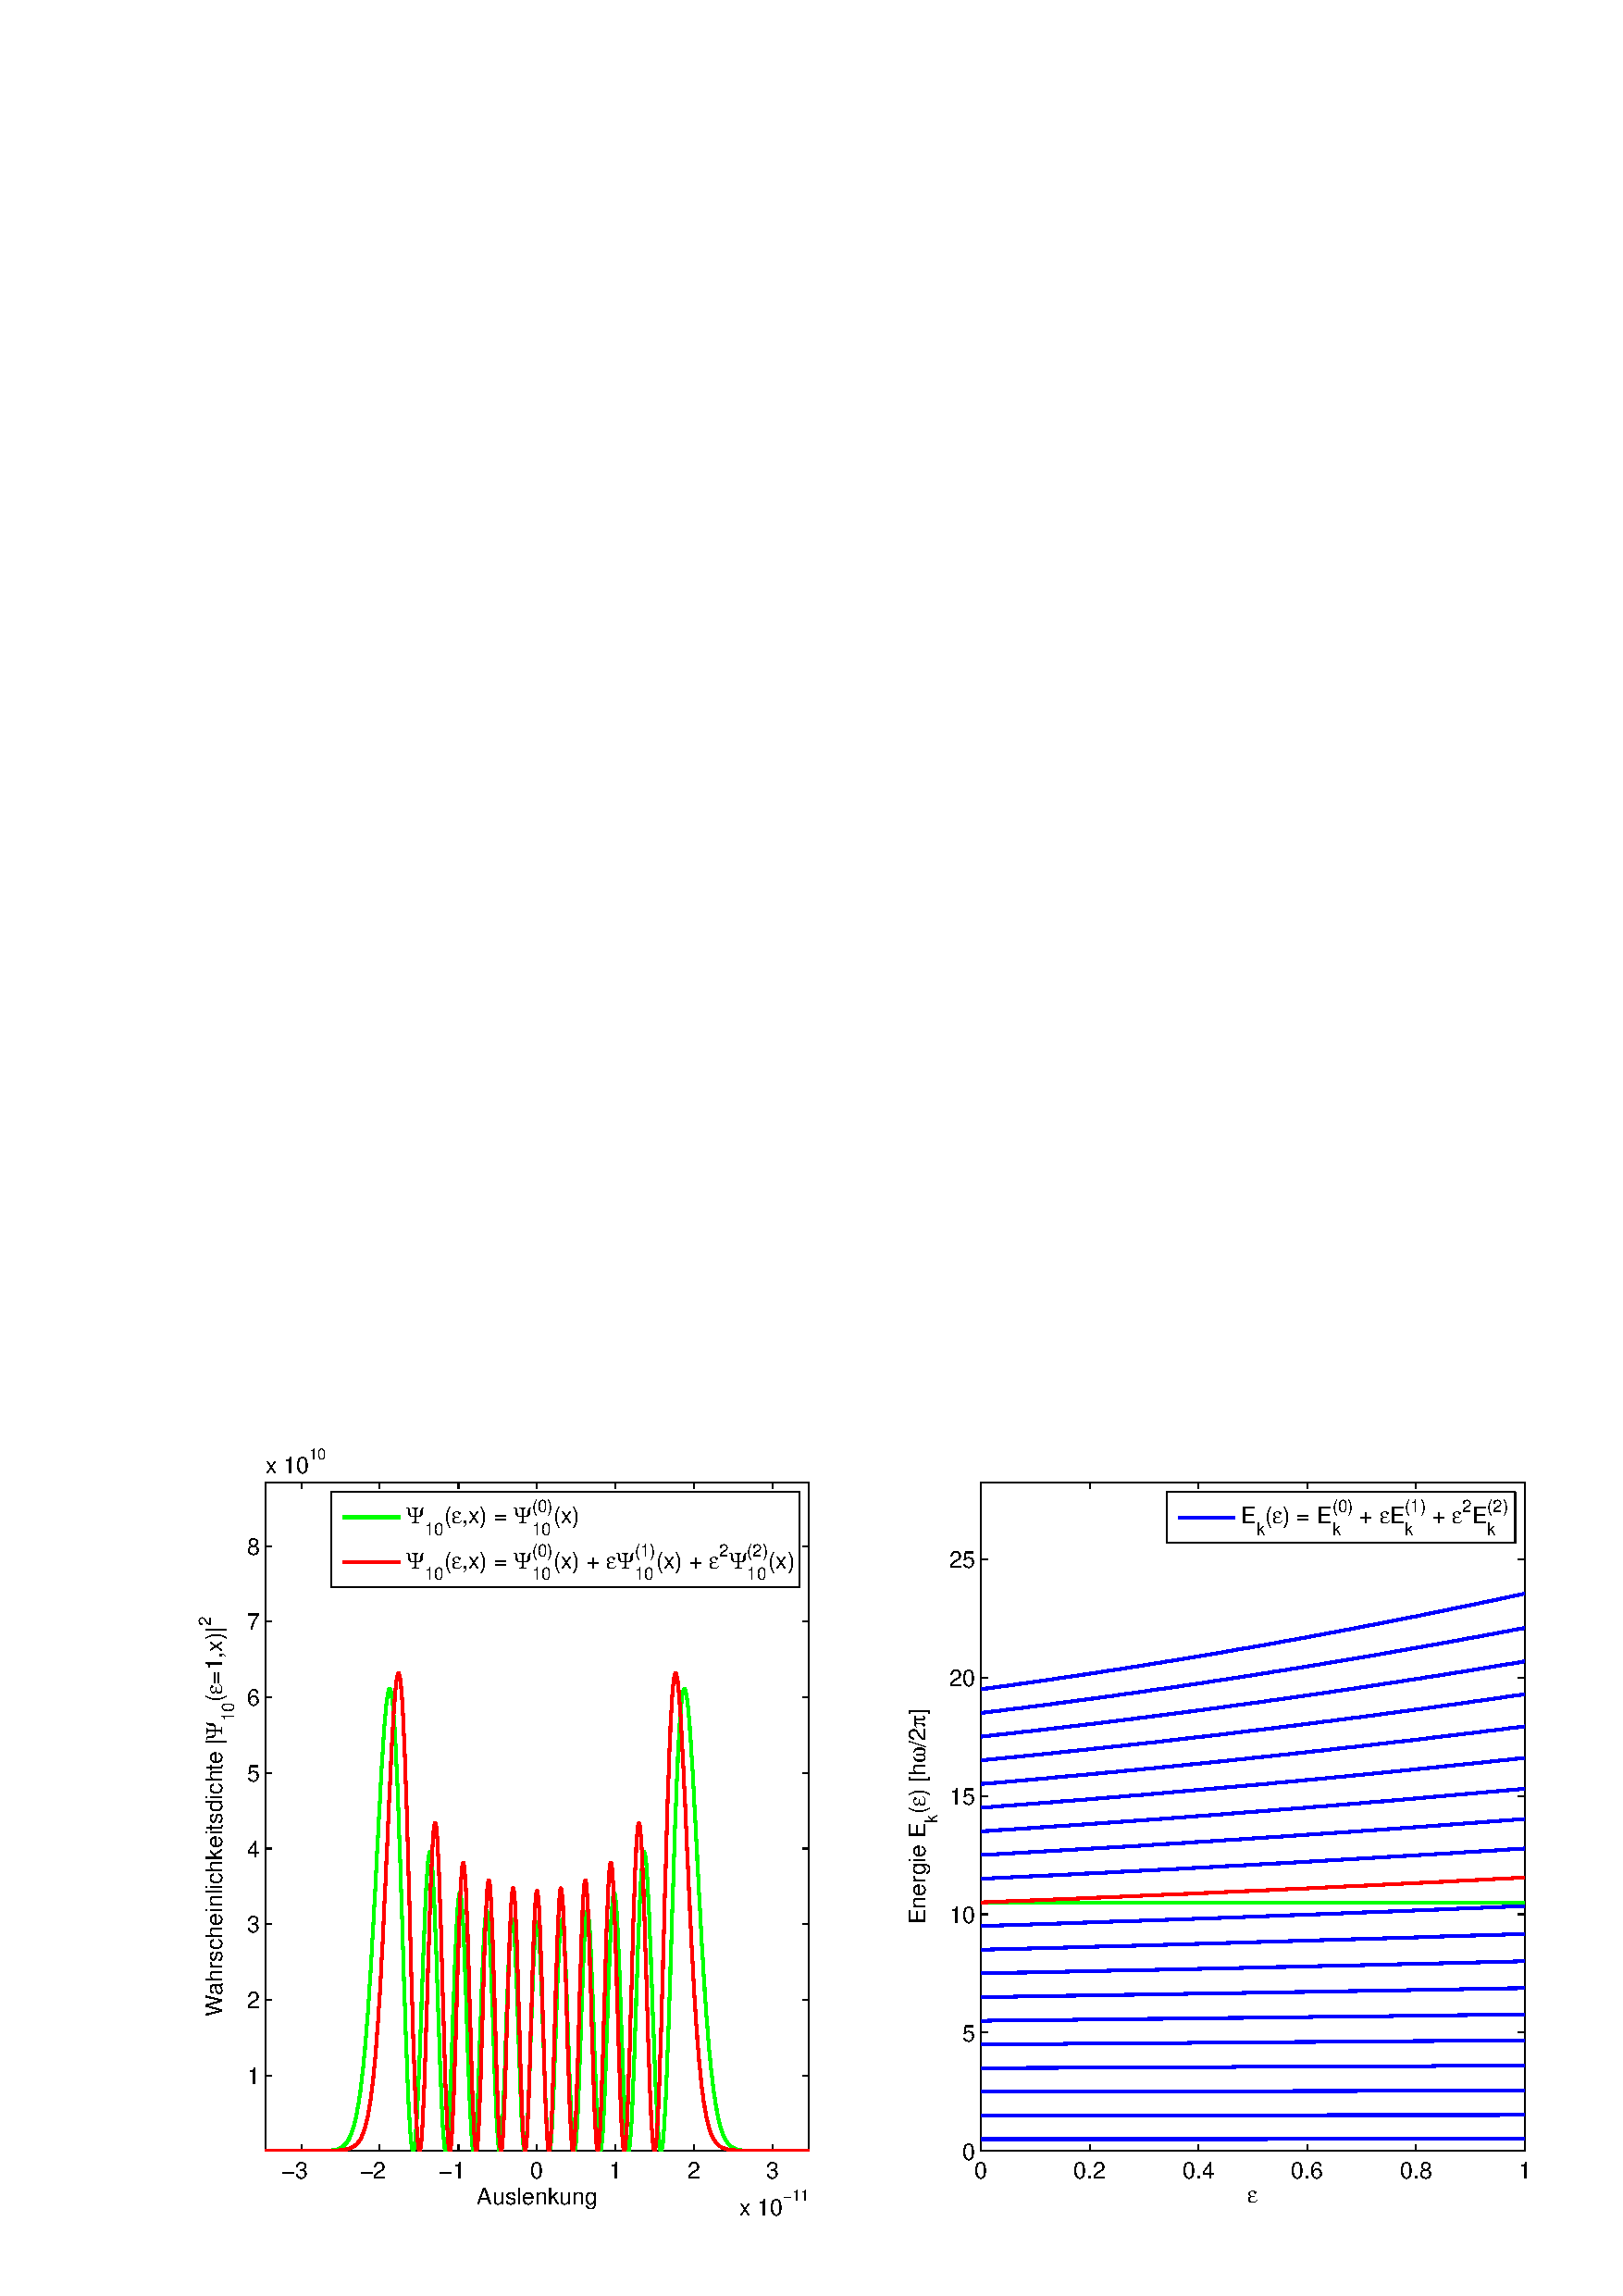
\includegraphics[width=0.8\textwidth]{anharmonisch/images/x4/Stoerung2Wellenfunktion.pdf}
\caption{$Q^4$ zweite N"aherung: 10. Wellenfunktion und Energieniveaus  
\label{skript:x4_Stoerung2Wellenfunktion}}
\end{figure}

Auf der Abbildung~\ref{skript:x4_Stoerung2Wellenfunktion} sieht man, dass die
Wellenfunktion wieder ein wenig zusammengedr"uckt wurde.
Aber in zweiter N"aherung beh"alt die Wellenfunktion ungef"ahr die Proportionen
der ungest"orten Wellenfunktion.
Bei den Energieniveaus kann man die Auswirkungen von $\varepsilon^2$ erkennen.

			%Zweites Beispiel
\subsection{Zweites Beispiel $Q^3$}

\begin{figure}	%Bild Stoerung1Skalare.pdf
\centering
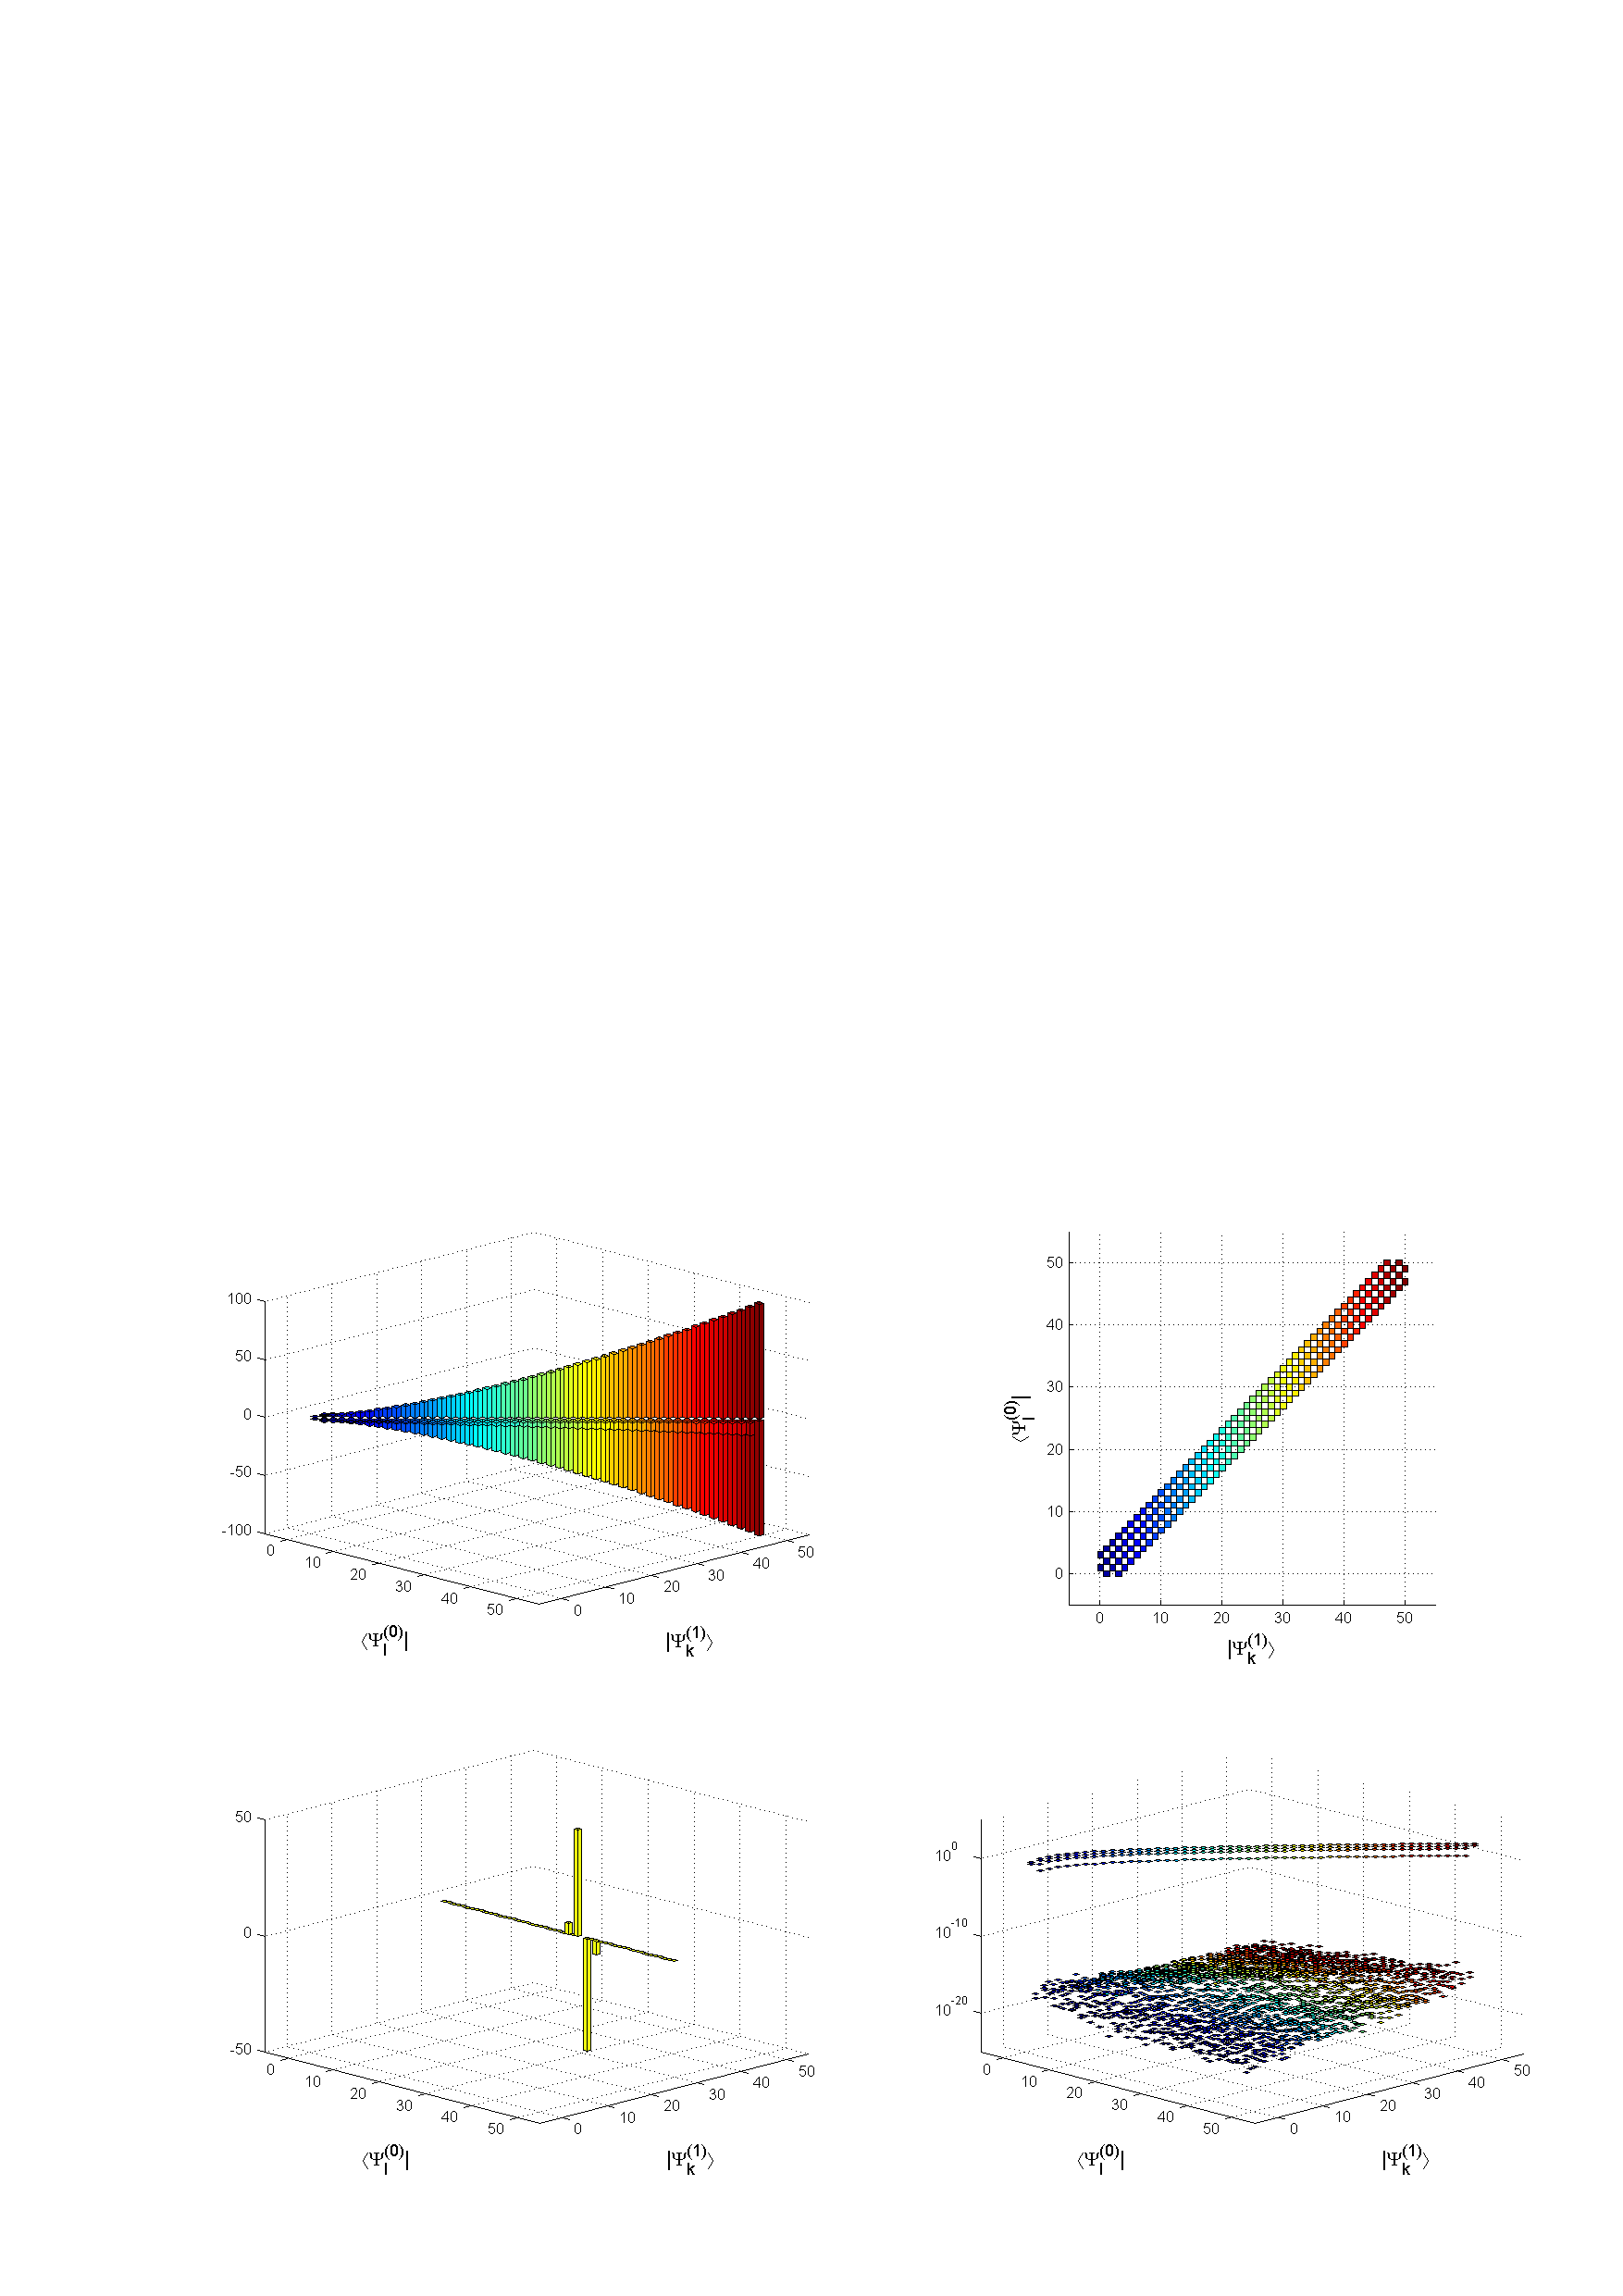
\includegraphics[width=1.0\textwidth]{anharmonisch/images/x3/Stoerung1Skalare.pdf}
\caption{$Q^3$ erste N"aherung: Skalarprodukte $\langle\Psi_l^{(0)}|\Psi_k^{(1)}\rangle$  
\label{skript:x3_Stoerung1Skalare}}
\end{figure}

Die Abbildung~\ref{skript:x3_Stoerung1Skalare} zeigt die erste N"aherung f"ur $Q^3$.
Dieses mal geben die Wellenfunktionen, bei welchen $l=k\pm 2,k\pm 4,\dots$ ist,
keinen Anteil an die gest"orte Wellenfunktion.
Ausserdem kann man sehen, dass die Anzahl an Wellenfunktionen $\Psi_l^{(0)}$,
welche einen Einfluss auf $\Psi_k^{(1)}$ kleiner ist als bei $Q^4$

\begin{figure}	%Bild EK1.pdf
\centering
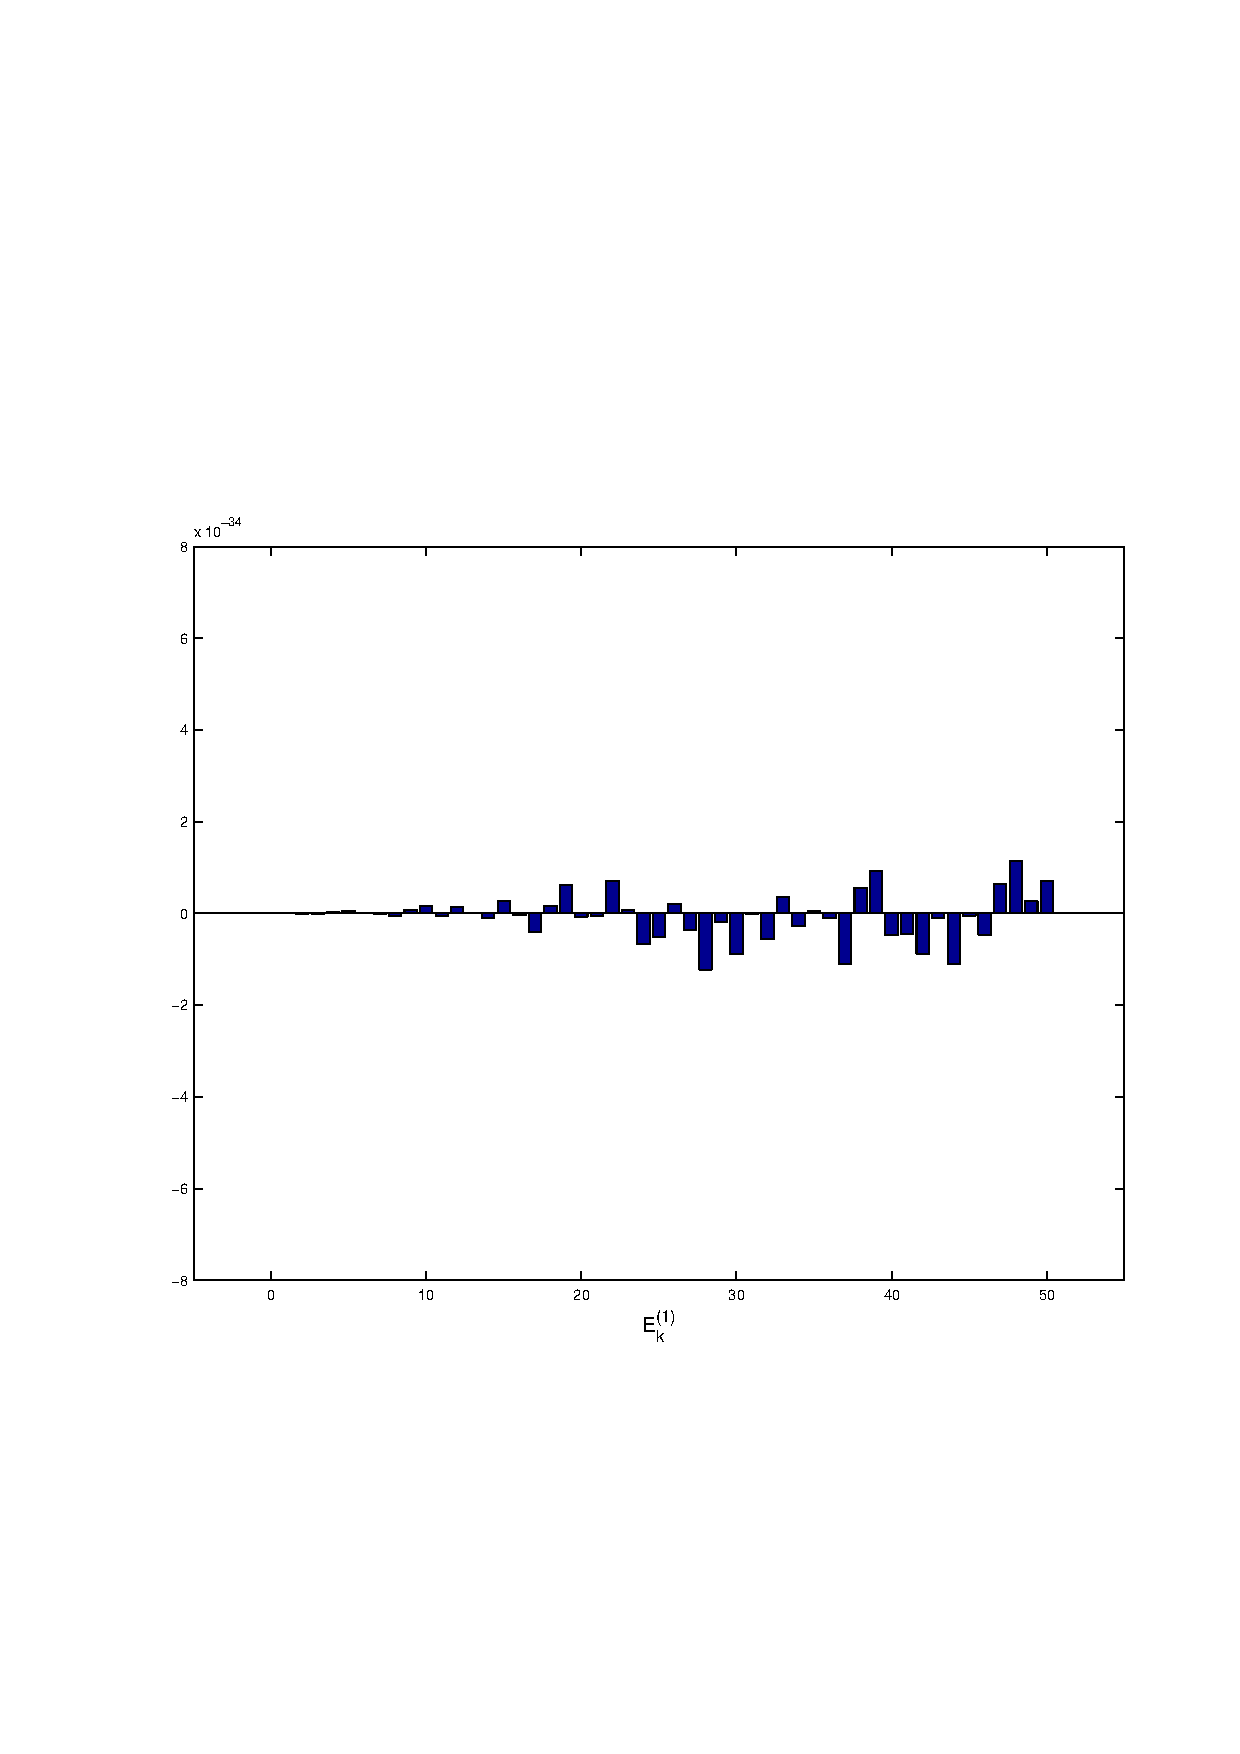
\includegraphics[width=0.7\textwidth]{anharmonisch/images/x3/EK1.pdf}
\caption{$Q^3$ erste N"aherung: St"orung der Energieniveaus  
\label{skript:x3_EK1}}
\end{figure}

Auf der Abbildung~\ref{skript:x3_EK1} sieht man, dass die "Anderungen
der Energieniveau gleich Null sind.
Wenn man die Gleichung~\ref{skript:stoerungsloesung1ordnung} betrachtet,
sieht man, dass eine gerade oder ungerade Wellenfunktion mit einem ungeraden
St"orterm multipliziert wird.
Daraus ergibt sich daraus wieder eine ungerade Funktion.
Wird diese Funktion aufsummiert,
l"oschen sich die positiven und negativen Anteile auf.

\begin{figure}	%Bild Stoerung1Wellenfunktion.pdf
\centering
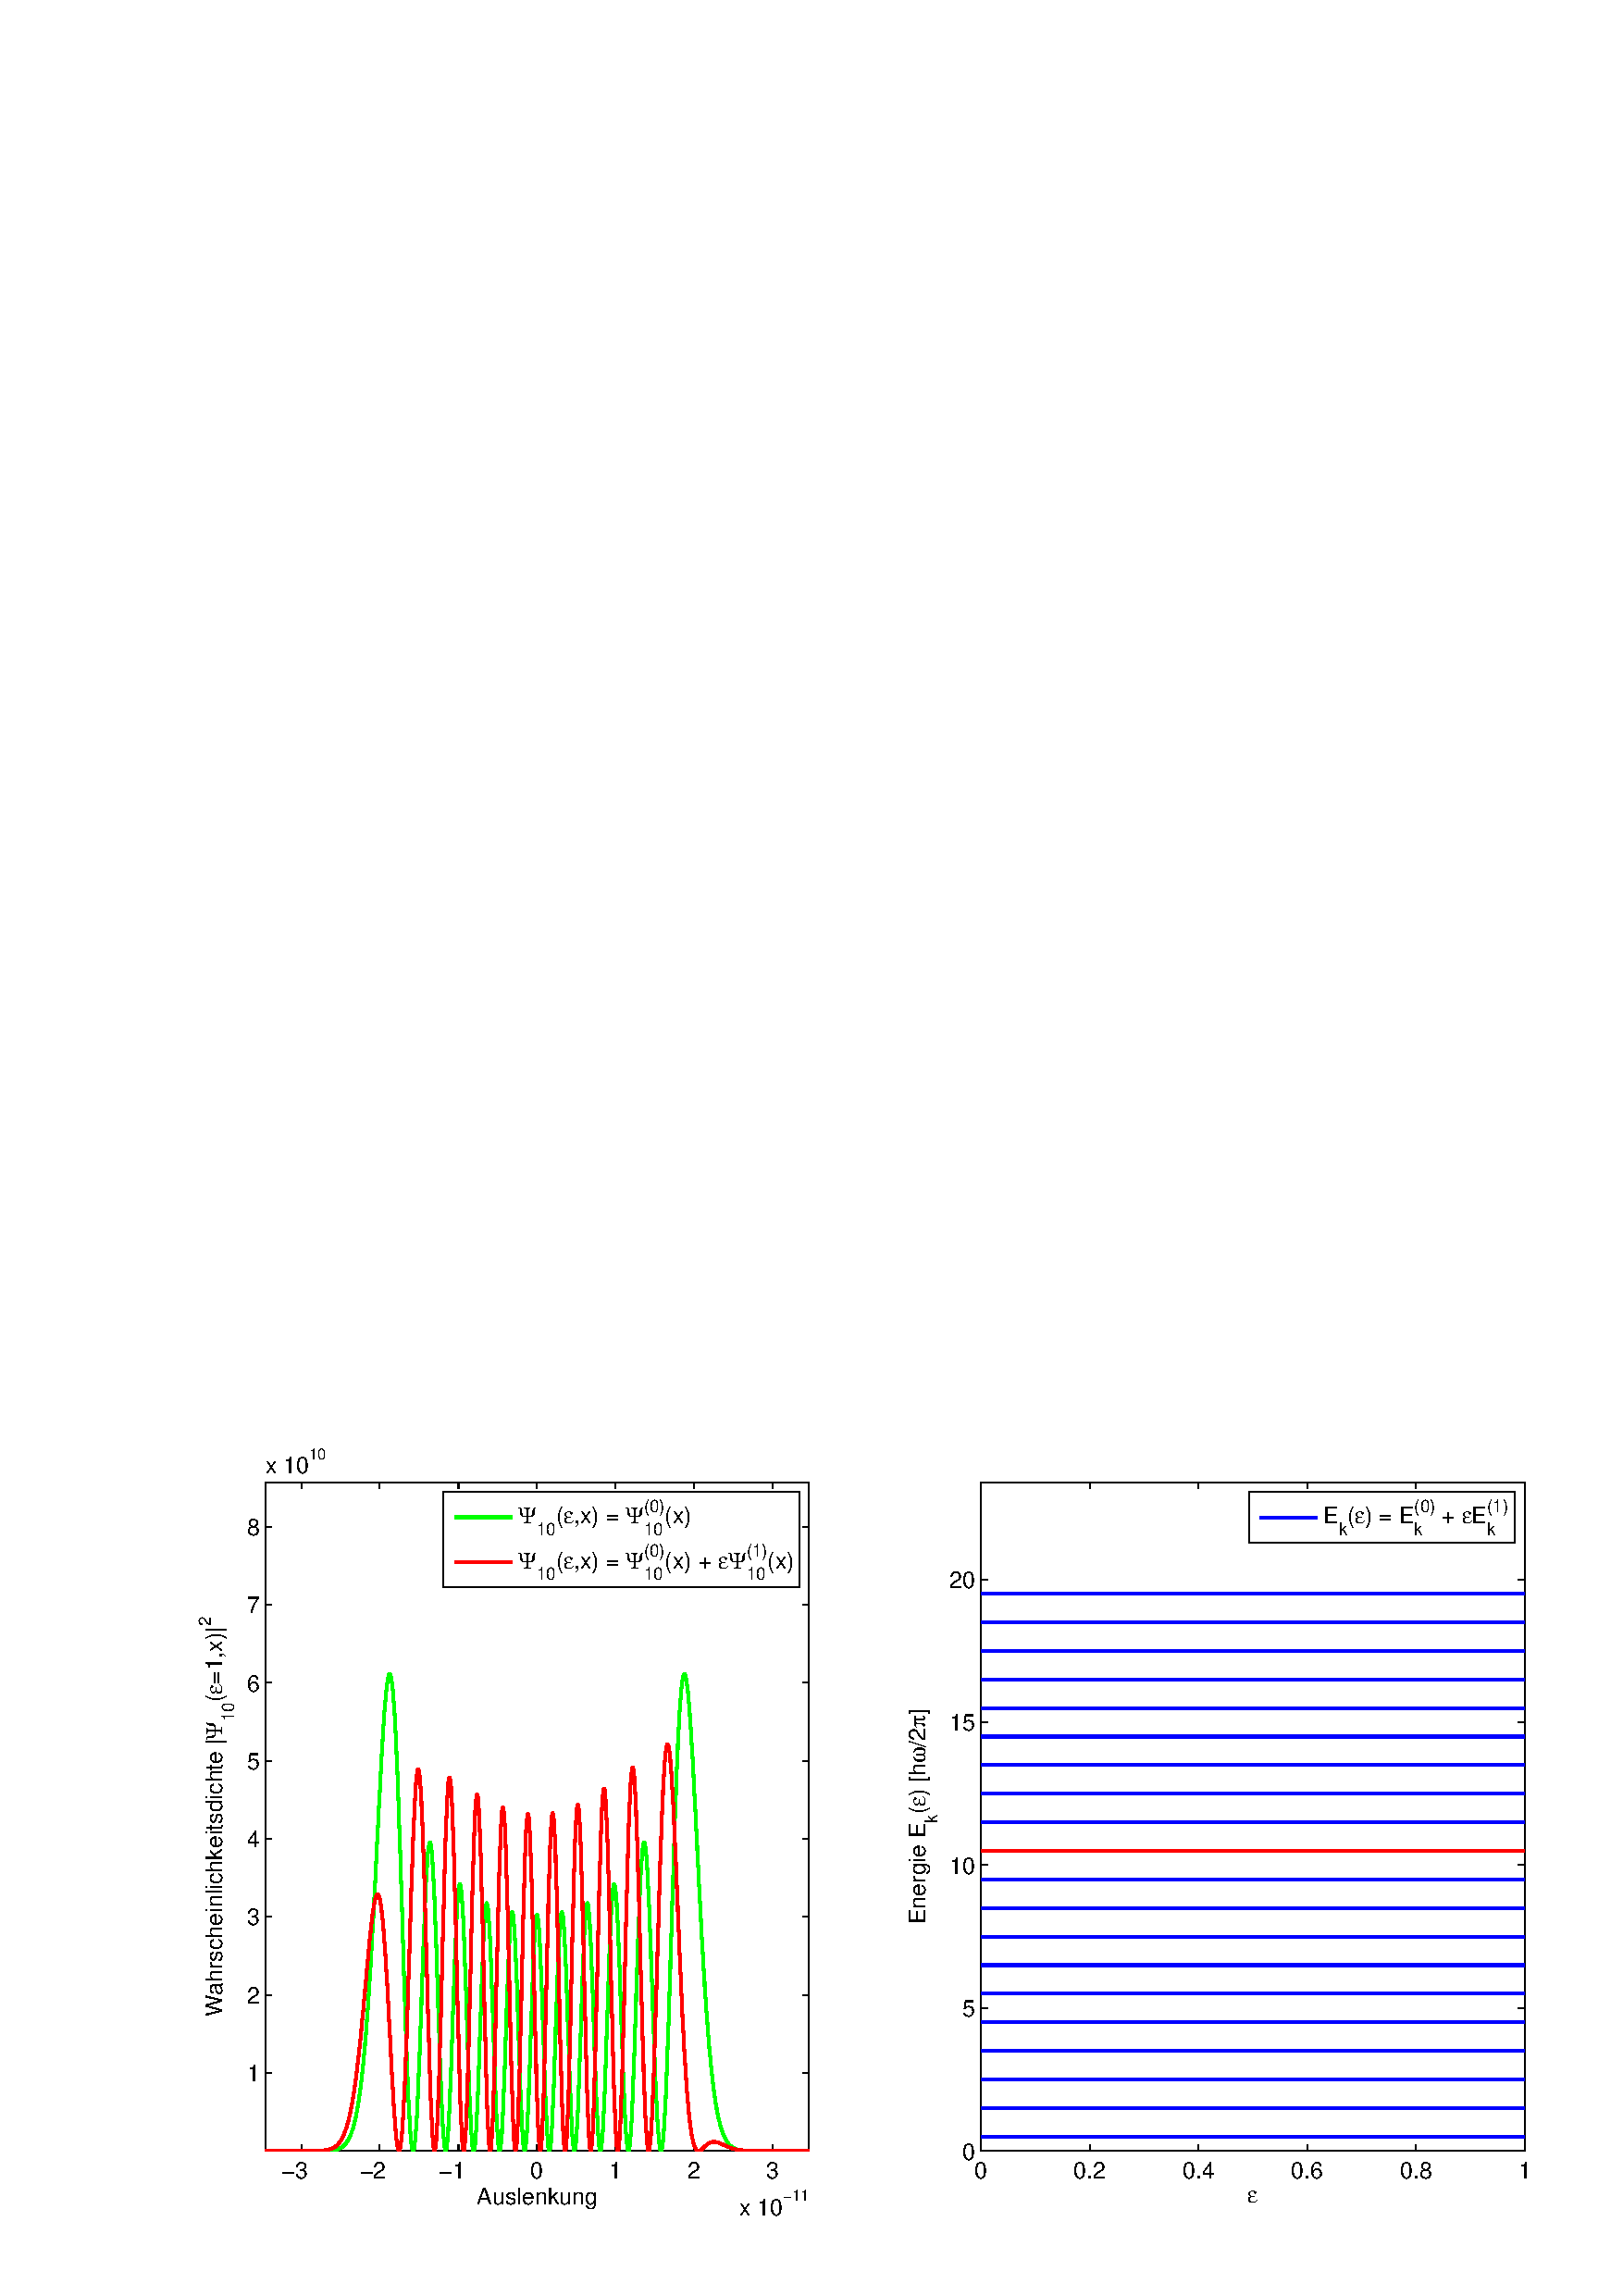
\includegraphics[width=0.8\textwidth]{anharmonisch/images/x3/Stoerung1Wellenfunktion.pdf}
\caption{$Q^3$ erste N"aherung: 10. Wellenfunktion und Energieniveaus 
\label{skript:x3_Stoerung1Wellenfunktion}}
\end{figure}

Auf der Abbildung~\ref{skript:x3_Stoerung1Wellenfunktion} sieht man,
dass die Wellenfunktion nach links verschoben wurde.
Das heisst, das ein Kraftfeld von rechts nach links auf das System wirkt.
Wie man auf Grund von Abbildung~\ref{skript:x3_EK1} erwarten konnte,
haben sich die Energieniveaus nicht ver"andert.

\begin{figure}	%Bild Stoerung2Skalare.pdf
\centering
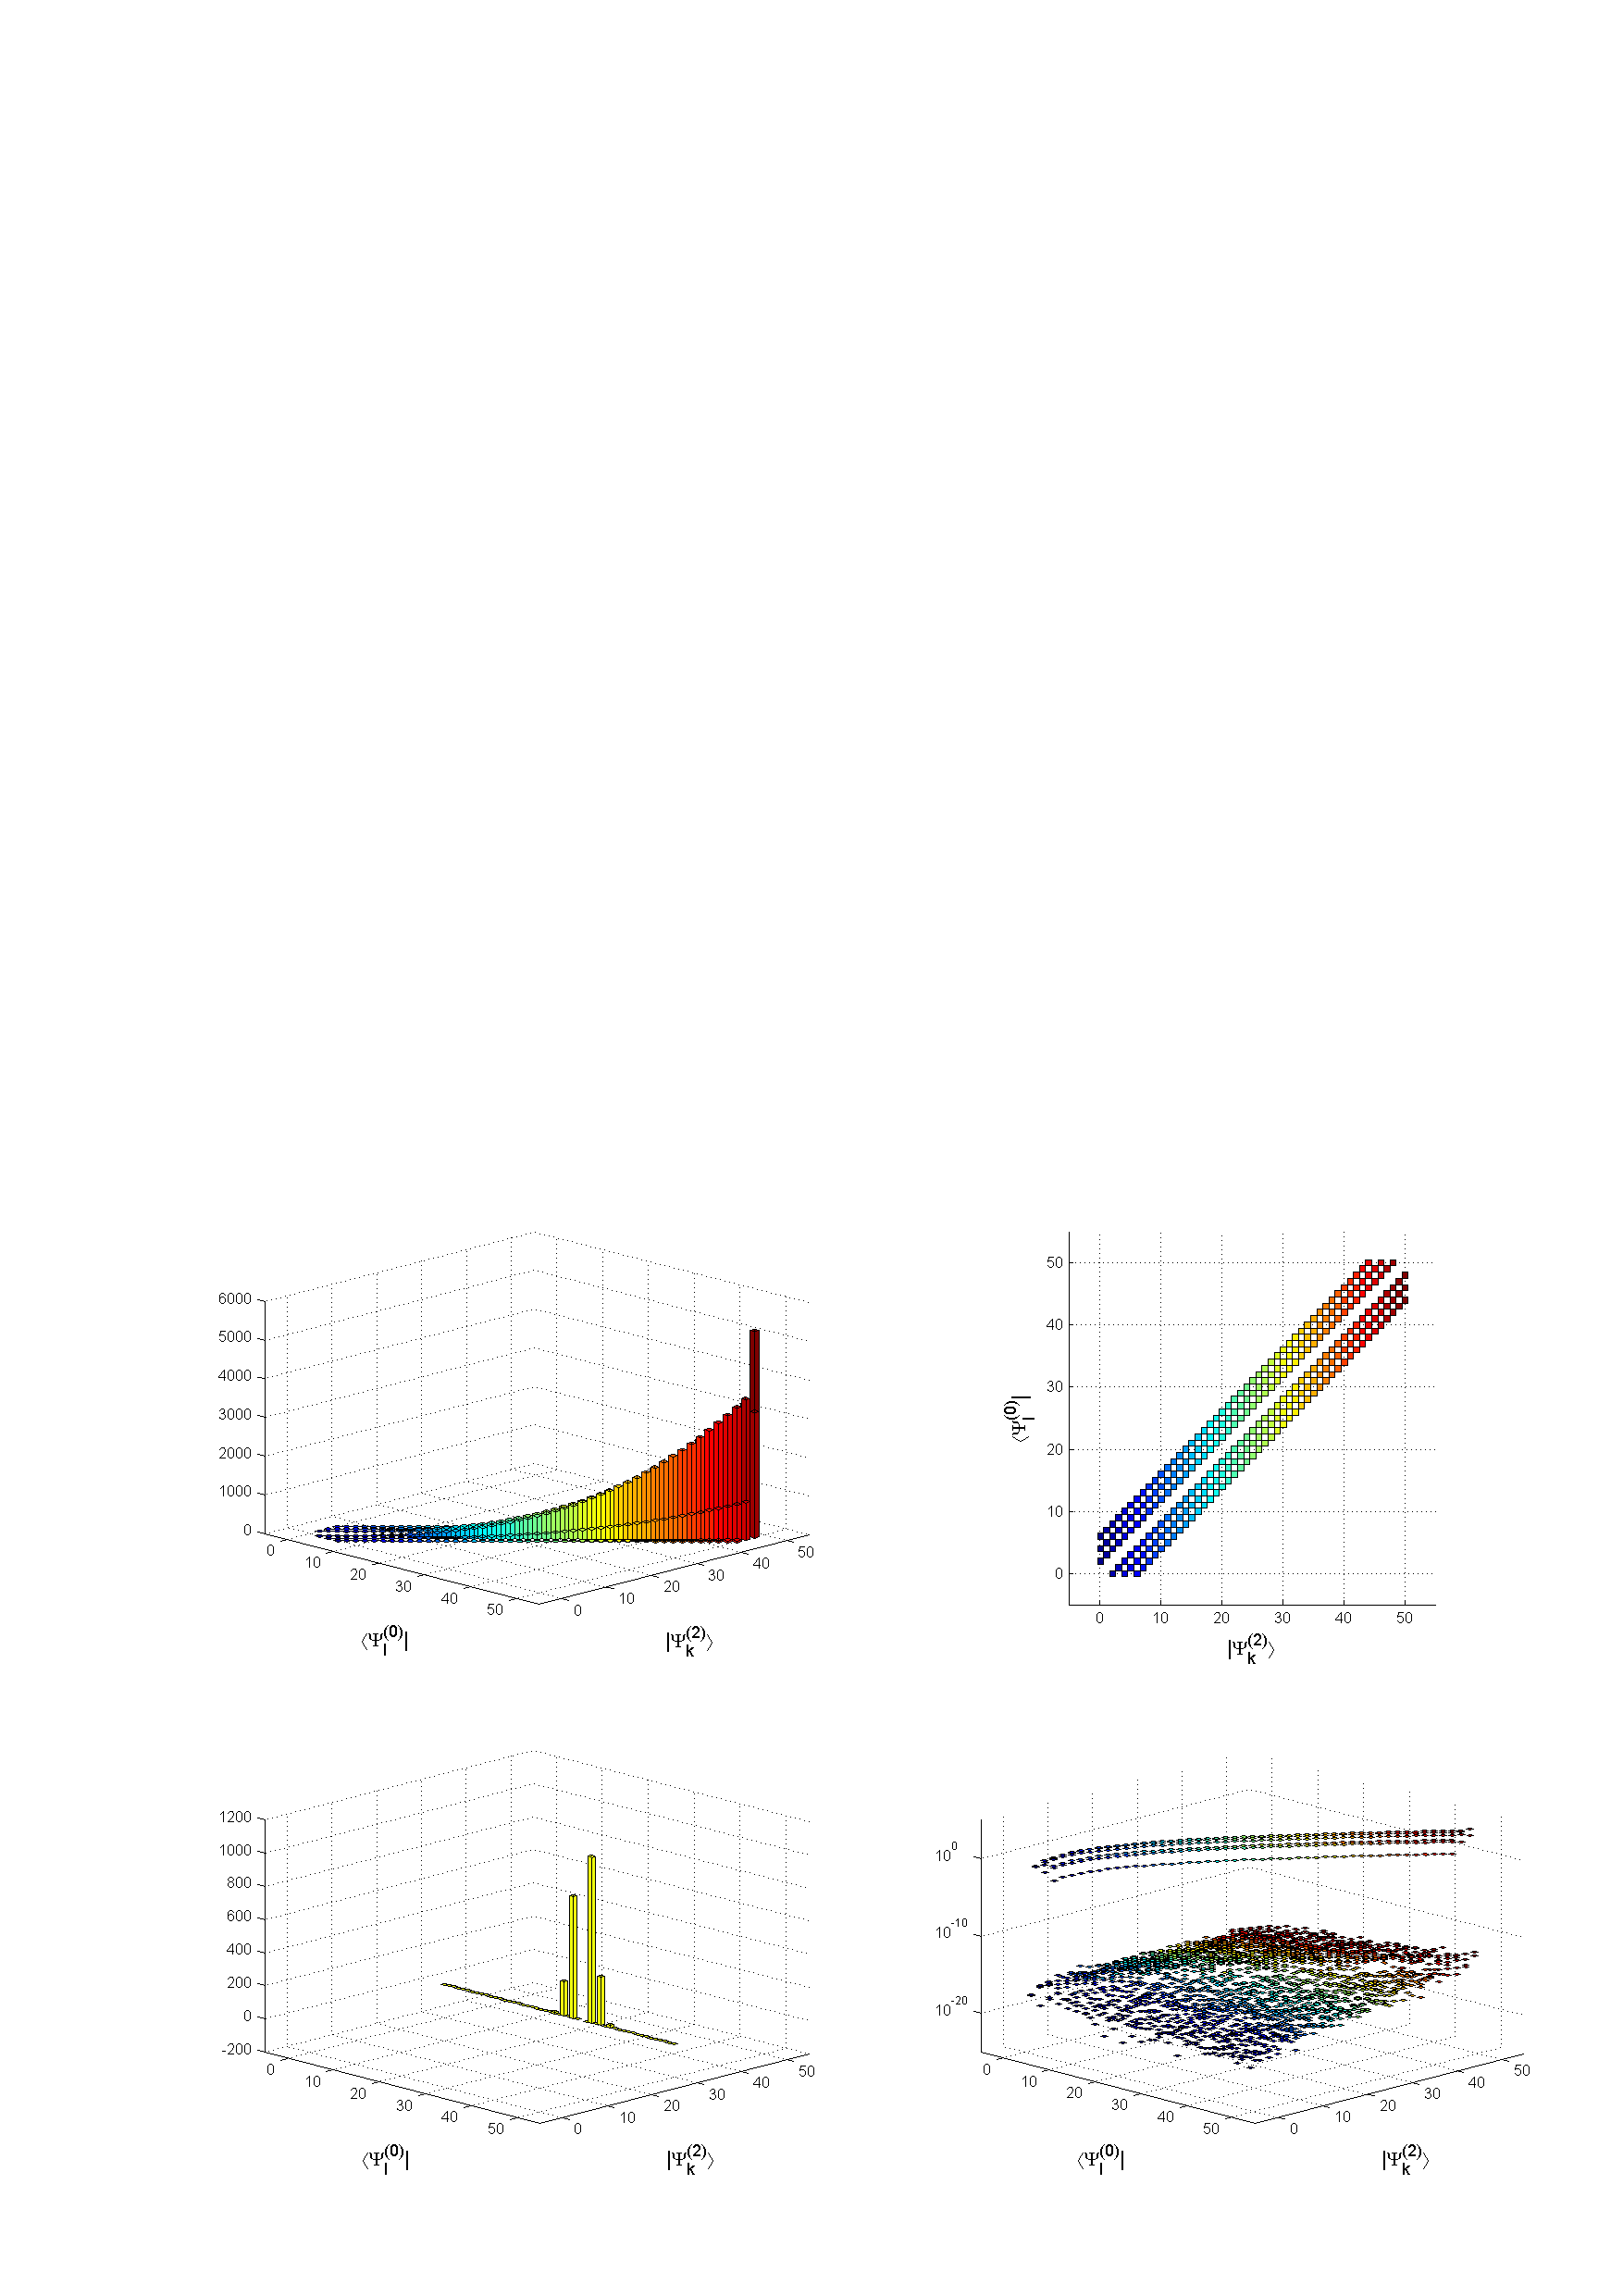
\includegraphics[width=1.0\textwidth]{anharmonisch/images/x3/Stoerung2Skalare.pdf}
\caption{$Q^3$ zweite N"aherung: Skalarprodukte $\langle\Psi_l^{(0)}|\Psi_k^{(2)}\rangle$ 
\label{skript:x3_Stoerung2Skalare}}
\end{figure}

Die Abbildung~\ref{skript:x3_Stoerung2Skalare} zeigt die zweite N"aherung f"ur $Q^3$.
Bei der zweiten N"aherung geben die Wellenfunktionen,
bei welchen $l=k\pm 1,k\pm 3,\dots$ ist,
keinen Anteil an die gest"orte Wellenfunktion.
Hier sieht man auch, dass alle Skalarprodukte positiv sind.

\begin{figure}	%Bild EK2.pdf
\centering
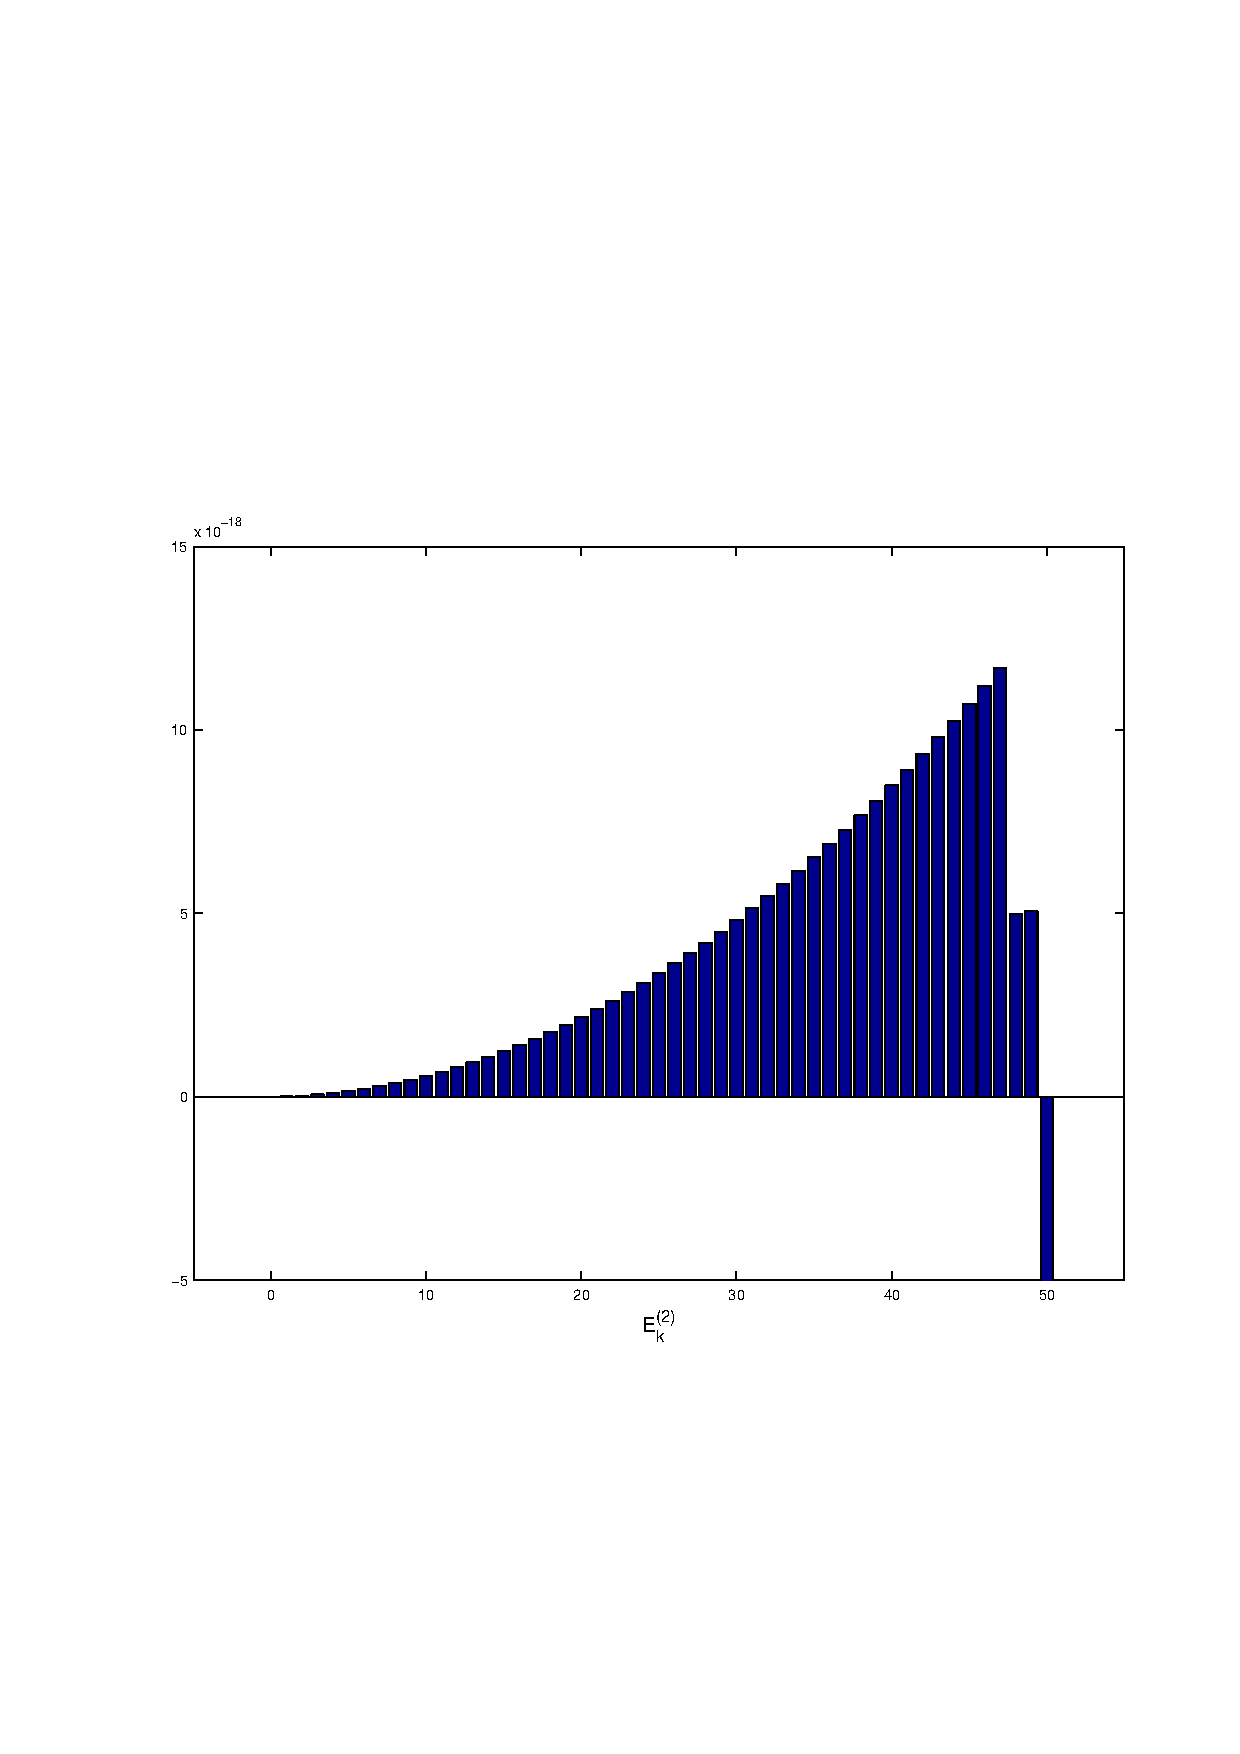
\includegraphics[width=0.7\textwidth]{anharmonisch/images/x3/EK2.pdf}
\caption{$Q^3$ zweite N"aherung: St"orung der Energieniveaus  
\label{skript:x3_EK2}}
\end{figure}

Auf der Abbildung~\ref{skript:x3_EK2} sieht man die "Anderung der Energieniveaus
in zweiter N"aherung.
Aus dem selben Grund wie schon bei $Q^4$, kann man auch hier diese Randeffekte
sehen.

\begin{figure}	%Bild Stoerung2Wellenfunktion.pdf
\centering
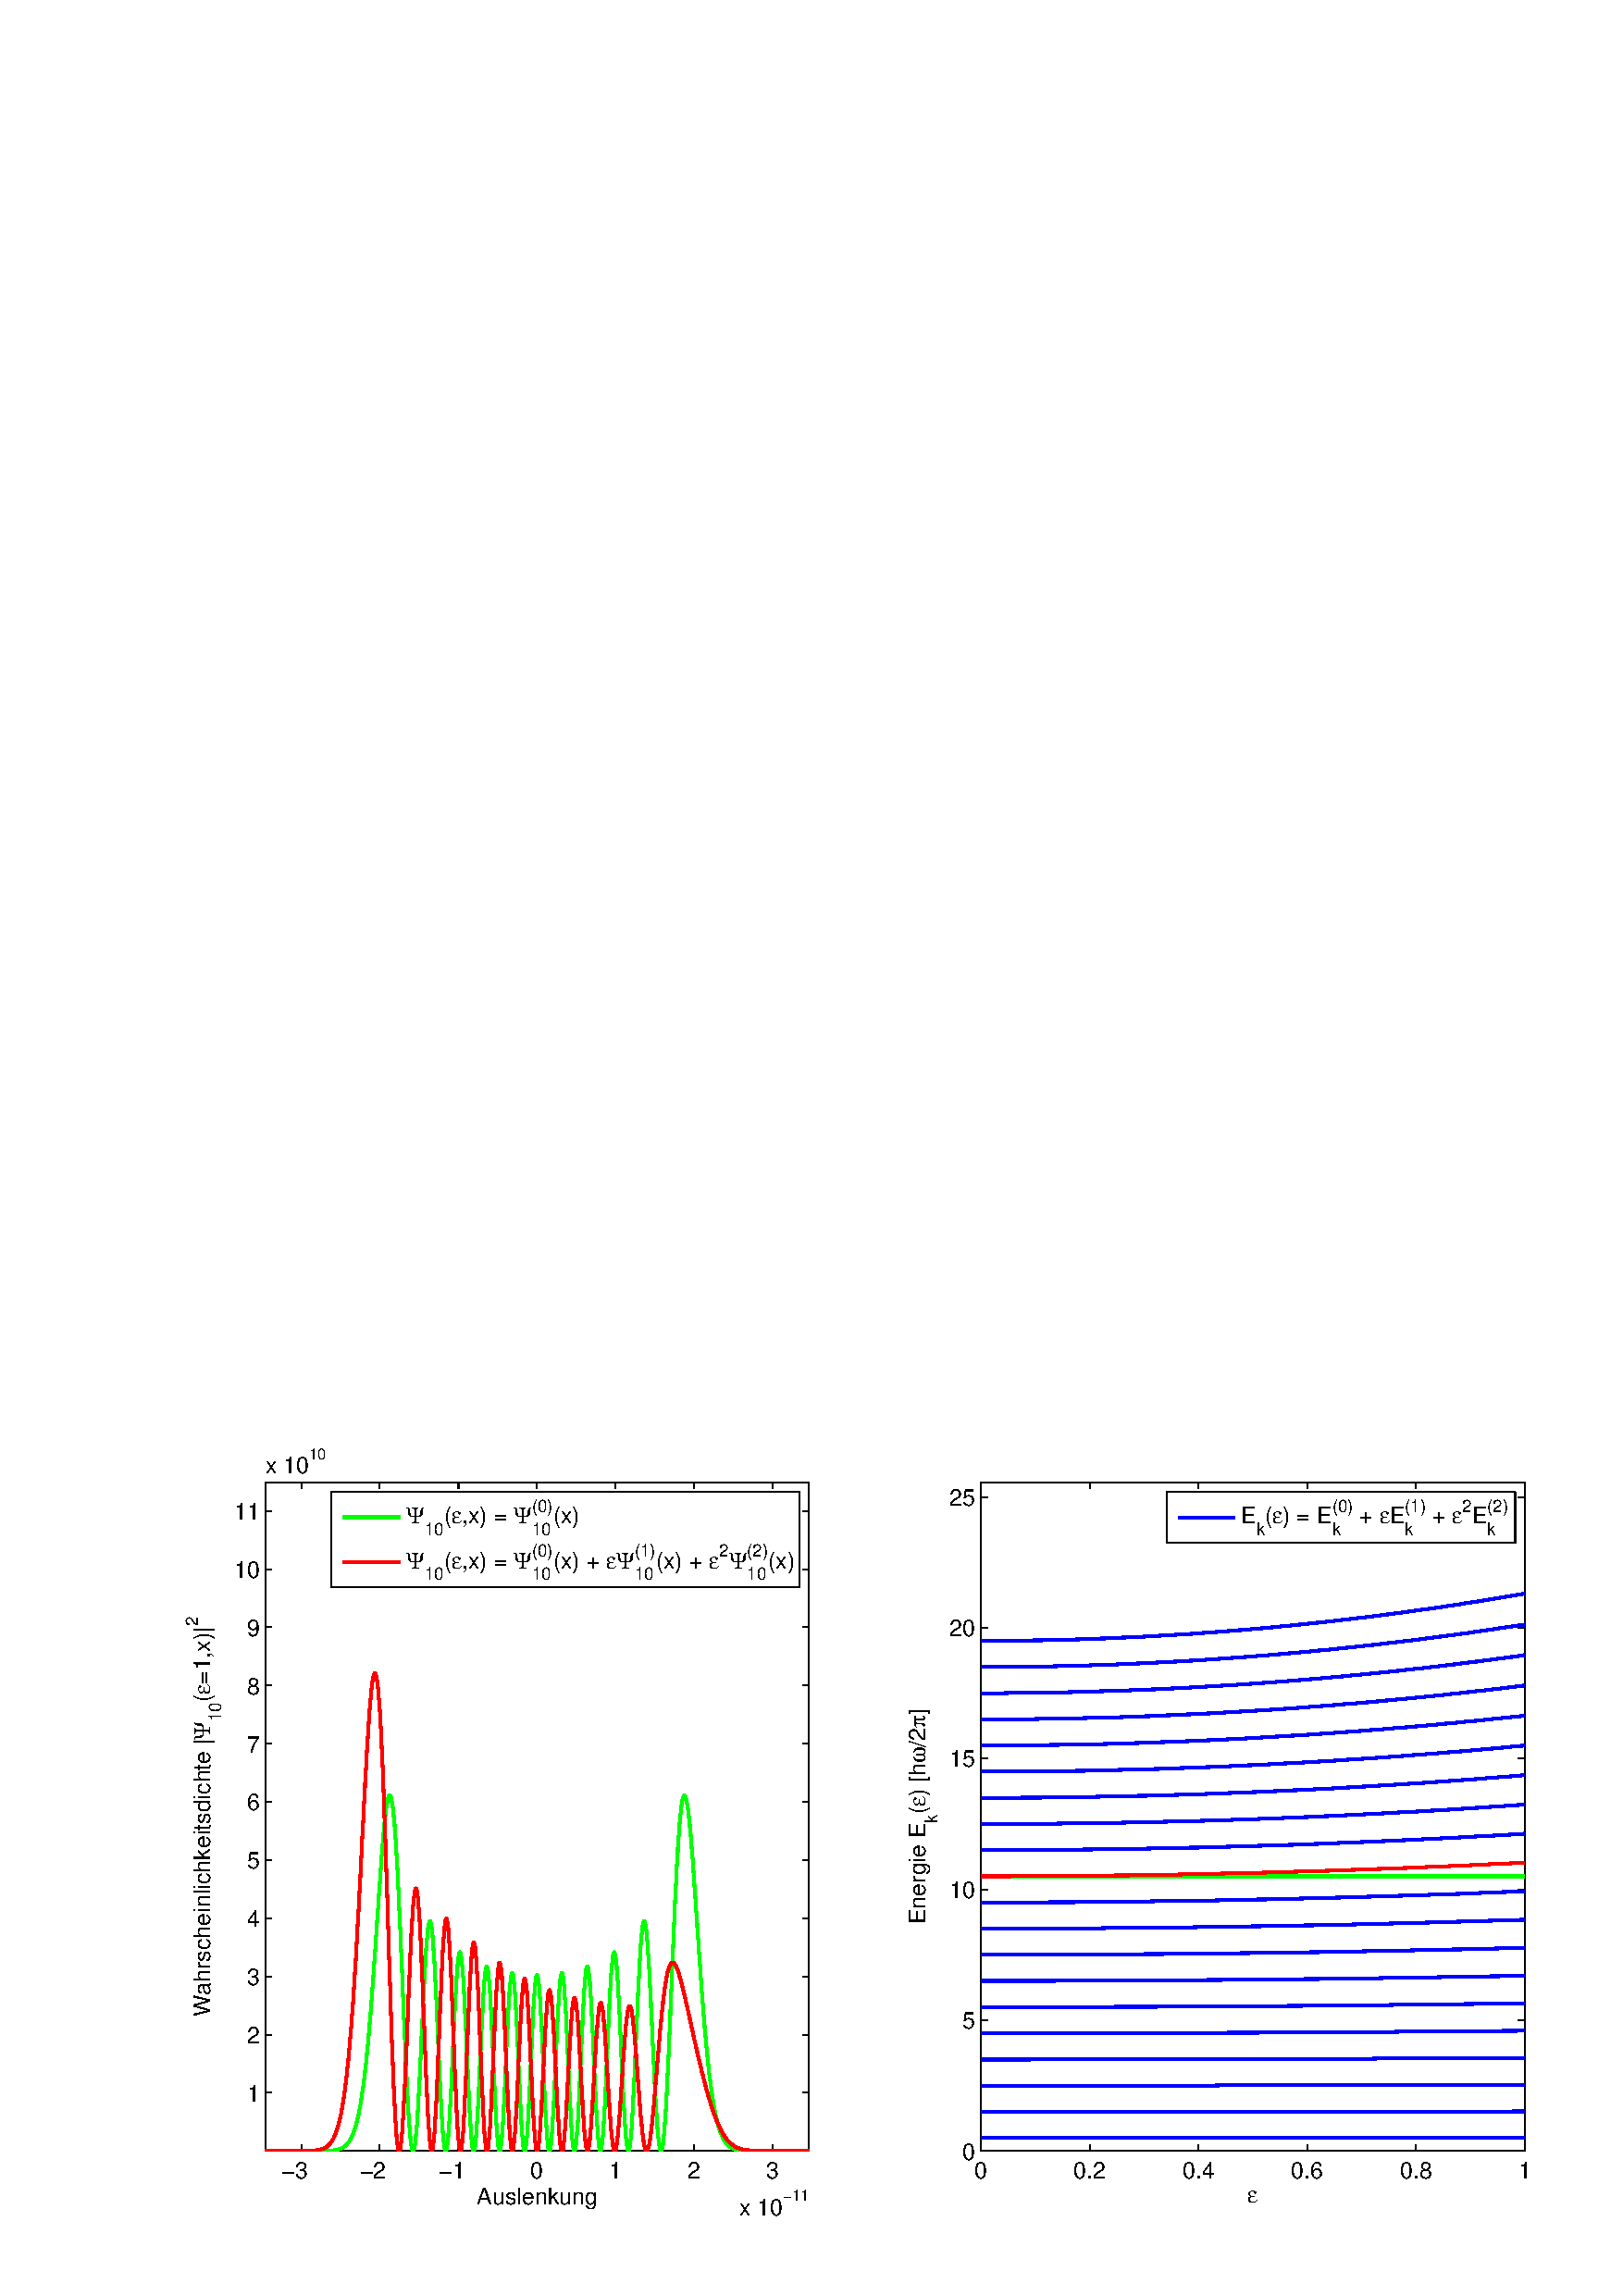
\includegraphics[width=0.8\textwidth]{anharmonisch/images/x3/Stoerung2Wellenfunktion.pdf}
\caption{$Q^3$ zweite N"aherung: 10. Wellenfunktion und Energieniveaus
\label{skript:x3_Stoerung1Wellenfunktion}}
\end{figure}

Auf der Abbildung~\ref{skript:x3_Stoerung2Wellenfunktion} sieht man,
dass die Verschiebung nach links noch st"arker Ausgepr"agt ist.
Die Energieniveaus verschieben sich in zweiter N"aherung auch wieder nach oben,
wie es auch bei $Q^4$ der Fall war.

			%Fazit
\section{Fazit}
\rhead{Fazit}

Nat"urliche Vorg"ange im Atomaren Bereich lassen sich nur schwer  beschreiben.
Die Bewegungen eines Teilchens sind sehr komplex.
In diesem Kapitel sind wir auf diese Thematik eingegangen.
Wir haben die bereits behandelte St"orungstheorie vertieft,
so dass wir auch komplexere (anharmonische) Vorg"ange n"aherungsweise
beschreiben k"onnen.
Wie ein Molek"ul, welches mit seinen diskreten Energieniveaus,
in seinen Freiheitsgraden oszilliert.
Dies ist ein wichtiger Grundbaustein der Spektroskopie.
Es k"onnen pr"azise Fingerabdr"ucke von Molek"ulkonfigurationen erstellt werden.
Je nach Freiheitsgrad kann ein Teilchen, Strahlung mit spezifischer Wellenl"ange
(Spektrallinien)  absorbieren und  emittieren.
Wenn man die Theorie noch weiter vertiefen m"ochte, wird man verstehen,
warum Materie W"arme abgeben und aufnehmen kann,
oder warum Schwefel gelb und Kohle schwarz ist.

\printbibliography[heading=subbibliography]
\end{refsection}

